\subsection{Ergänzende Evaluation auf TextComplexityDE (Naderi et al., 2019)}
\label{sec:anhang_textcomplexityde}

In diesem Abschnitt sind die ergänzenden empirischen Auswertungen zur Satzkomplexitäts-Evaluation auf dem \textit{TextComplexityDE}-Benchmark \citep{naderi2019textcomplexityde} ($N = 1.000$ deutsche Wikipedia-Sätze mit menschlichen Likert-Urteilen) dargestellt.

\begin{table}[htbp]
\centering
\small
\caption{Gesamtevaluation aller Modellfamilien auf dem TextComplexityDE-Benchmark ($N = 1.000$ Sätze).}
\label{tab:anhang_textcomplexityde_master}
\adjustbox{max width=\textwidth}{%
\begin{tabular}{@{}llcccc@{}}
\toprule
\textbf{Modell} & \textbf{Kategorie} & \textbf{Pearson $r$ (Simplicity)} & \textbf{Spearman $\rho$ (Rang)} & \textbf{Kendall $\tau$} & \textbf{MAE (normiert)} \\
\midrule
LIX Lesbarkeitsindex                & Baseline             & $0{,}657$ & $0{,}641$ & $0{,}467$ & $0{,}177$ \\
BiLSTM Satz-Klassifikator          & Klassifikator (Satz) & $0{,}549$ & $\mathbf{0{,}648}$ & $0{,}468$ & $0{,}509$ \\
BiLSTM MixUp Regressor ($512$)     & Regressor ($512$)    & $0{,}583$ & $0{,}615$ & $0{,}446$ & $0{,}471$ \\
BiLSTM Artikel-Klassifikator ($512$)& Klassifikator ($512$)& $\mathbf{0{,}602}$ & $0{,}585$ & $0{,}417$ & $0{,}343$ \\
BiLSTM MixUp Regressor ($256$)     & Regressor ($256$)    & $0{,}567$ & $0{,}509$ & $0{,}361$ & $0{,}477$ \\
Wiener Sachtextformel              & Baseline             & $0{,}540$ & $0{,}519$ & $0{,}370$ & $0{,}164$ \\
BiLSTM MixUp Regressor ($1.024$)   & Regressor ($1.024$)  & $0{,}566$ & $0{,}461$ & $0{,}323$ & $0{,}464$ \\
Flesch Reading Ease                & Baseline             & $0{,}456$ & $0{,}456$ & $0{,}322$ & $0{,}174$ \\
BiLSTM Artikel-Klassifikator ($256$)& Klassifikator ($256$)& $0{,}394$ & $0{,}227$ & $0{,}151$ & $0{,}576$ \\
BiLSTM Artikel-Klassifikator ($1.024$)& Klassifikator ($1.024$)& $0{,}417$ & $0{,}193$ & $0{,}128$ & $0{,}557$ \\
\bottomrule
\end{tabular}}
\end{table}

\begin{figure}[htbp]
\centering

\includegraphics[width=0.95\textwidth]{images/textcomplexityde_correlation_barchart.png}
\caption{Pearson- und Spearman-Korrelationen aller Modelle mit dem menschlichen Einfachheitsurteil auf TextComplexityDE ($N = 1.000$ Sätze).}
\label{fig:anhang_textcomplexityde_barchart}
\end{figure}

\begin{figure}[htbp]
\centering

\includegraphics[width=\textwidth]{images/textcomplexityde_scatter_all_models_grid.png}
\caption{Streudiagramm-Grid aller 10 Modellvarianten gegen den kontinuierlichen menschlichen Einfachheits-Score auf TextComplexityDE inklusive Regressionsgeraden.}
\label{fig:anhang_textcomplexityde_scatter}
\end{figure}

\begin{figure}[htbp]
\centering

\includegraphics[width=\textwidth]{images/textcomplexityde_boxplots_all_models_grid.png}
\caption{Boxplot-Verteilungen der Modell-Scores gruppiert nach den diskretisierten Likert-Komplexitätsstufen auf TextComplexityDE.}
\label{fig:anhang_textcomplexityde_boxplots}
\end{figure}

\newpage
\subsection{Ergänzende Evaluation auf dem MERLIN CEFR-Benchmark (Boyd et al., 2014)}
\label{sec:anhang_merlin}

In diesem Abschnitt sind die detaillierten statistischen Auswertungen zur Dokumenten- und Fließtextevaluation auf dem \textit{MERLIN}-Korpus \citep{boyd2014merlin} ($N = 1.033$ deutsche Volltexte mit offiziellen CEFR-Niveaustufen $A1$ bis $C2$) dokumentiert.

\begin{table}[htbp]
\centering
\small
\caption{Gesamtevaluation aller Modellfamilien auf dem MERLIN CEFR-Benchmark ($N = 1.033$ Dokumente).}
\label{tab:anhang_merlin_master}
\adjustbox{max width=\textwidth}{%
\begin{tabular}{@{}llcccc@{}}
\toprule
\textbf{Modell} & \textbf{Kategorie} & \textbf{Pearson $r$ (Simplicity)} & \textbf{Spearman $\rho$ (Rang)} & \textbf{Kendall $\tau$} & \textbf{MAE (normiert)} \\
\midrule
LIX Lesbarkeitsindex                & Baseline             & $\mathbf{0{,}632}$ & $\mathbf{0{,}656}$ & $0{,}515$ & $0{,}127$ \\
Wiener Sachtextformel              & Baseline             & $0{,}584$ & $0{,}602$ & $0{,}463$ & $0{,}137$ \\
Flesch Reading Ease                & Baseline             & $0{,}513$ & $0{,}543$ & $0{,}412$ & $0{,}144$ \\
BiLSTM Artikel-Klassifikator ($512$)& Klassifikator ($512$)& $\mathbf{0{,}386}$ & $0{,}397$ & $0{,}296$ & $0{,}408$ \\
BiLSTM MixUp Regressor ($512$)     & Regressor ($512$)    & $0{,}348$ & $0{,}352$ & $0{,}268$ & $0{,}346$ \\
BiLSTM MixUp Regressor ($1.024$)   & Regressor ($1.024$)  & $0{,}327$ & $0{,}328$ & $0{,}251$ & $0{,}347$ \\
BiLSTM MixUp Regressor ($256$)     & Regressor ($256$)    & $0{,}304$ & $0{,}296$ & $0{,}226$ & $0{,}341$ \\
BiLSTM Satz-Klassifikator          & Klassifikator (Satz) & $0{,}285$ & $\mathbf{0{,}419}$ & $0{,}319$ & $0{,}483$ \\
BiLSTM Artikel-Klassifikator ($256$)& Klassifikator ($256$)& $0{,}076$ & $0{,}518$ & $0{,}389$ & $0{,}566$ \\
BiLSTM Artikel-Klassifikator ($1.024$)& Klassifikator ($1.024$)& $-0{,}049$ & $-0{,}078$ & $-0{,}058$ & $0{,}569$ \\
\bottomrule
\end{tabular}}
\end{table}

\begin{table}[htbp]
\centering
\small
\caption{Mittelwerte der vorhergesagten Modell-Scores über die 6 CEFR-Stufen im MERLIN-Korpus zur Überprüfung der Monotonie ($A1 \to C2$).}
\label{tab:anhang_merlin_monotonie}
\adjustbox{max width=\textwidth}{%
\begin{tabular}{@{}lcccccc@{}}
\toprule
\textbf{CEFR-Stufe} & \shortstack{\textbf{MixUp Reg.}\\\textbf{($256$)}} & \shortstack{\textbf{MixUp Reg.}\\\textbf{($512$)}} & \shortstack{\textbf{MixUp Reg.}\\\textbf{($1.024$)}} & \shortstack{\textbf{Art.-Klass.}\\\textbf{($512$)}} & \shortstack{\textbf{Satz-Klass.}\\\textbf{(P(LS))}} & \shortstack{\textbf{Wiener}\\\textbf{Formel}} \\
\midrule
\textbf{A1} (Sehr einfach, $N=57$)   & $0{,}2957$ & $0{,}3353$ & $0{,}3368$ & $\mathbf{0{,}5042}$ & $0{,}3043$ & $-1{,}28$ \\
\textbf{A2} (Einfach, $N=306$)       & $0{,}3302$ & $0{,}3356$ & $0{,}3596$ & $\mathbf{0{,}4419}$ & $0{,}2537$ & $-1{,}52$ \\
\textbf{B1} (Mittelstufe, $N=331$)   & $0{,}2966$ & $0{,}2946$ & $0{,}3166$ & $\mathbf{0{,}3385}$ & $0{,}1624$ & $-2{,}38$ \\
\textbf{B2} (Fortgeschritten, $N=293$)& $0{,}1944$ & $0{,}1762$ & $0{,}2017$ & $\mathbf{0{,}0955}$ & $0{,}0607$ & $-4{,}57$ \\
\textbf{C1} (Fachsprache, $N=42$)    & $0{,}1241$ & $0{,}1011$ & $0{,}1055$ & $\mathbf{0{,}0730}$ & $0{,}0751$ & $-5{,}30$ \\
\textbf{C2} (Muttersprachlich, $N=4$)& $0{,}0762$ & $0{,}0686$ & $0{,}0692$ & $\mathbf{0{,}0499}$ & $0{,}0334$ & $-5{,}24$ \\
\bottomrule
\end{tabular}}
\end{table}

\begin{figure}[htbp]
\centering
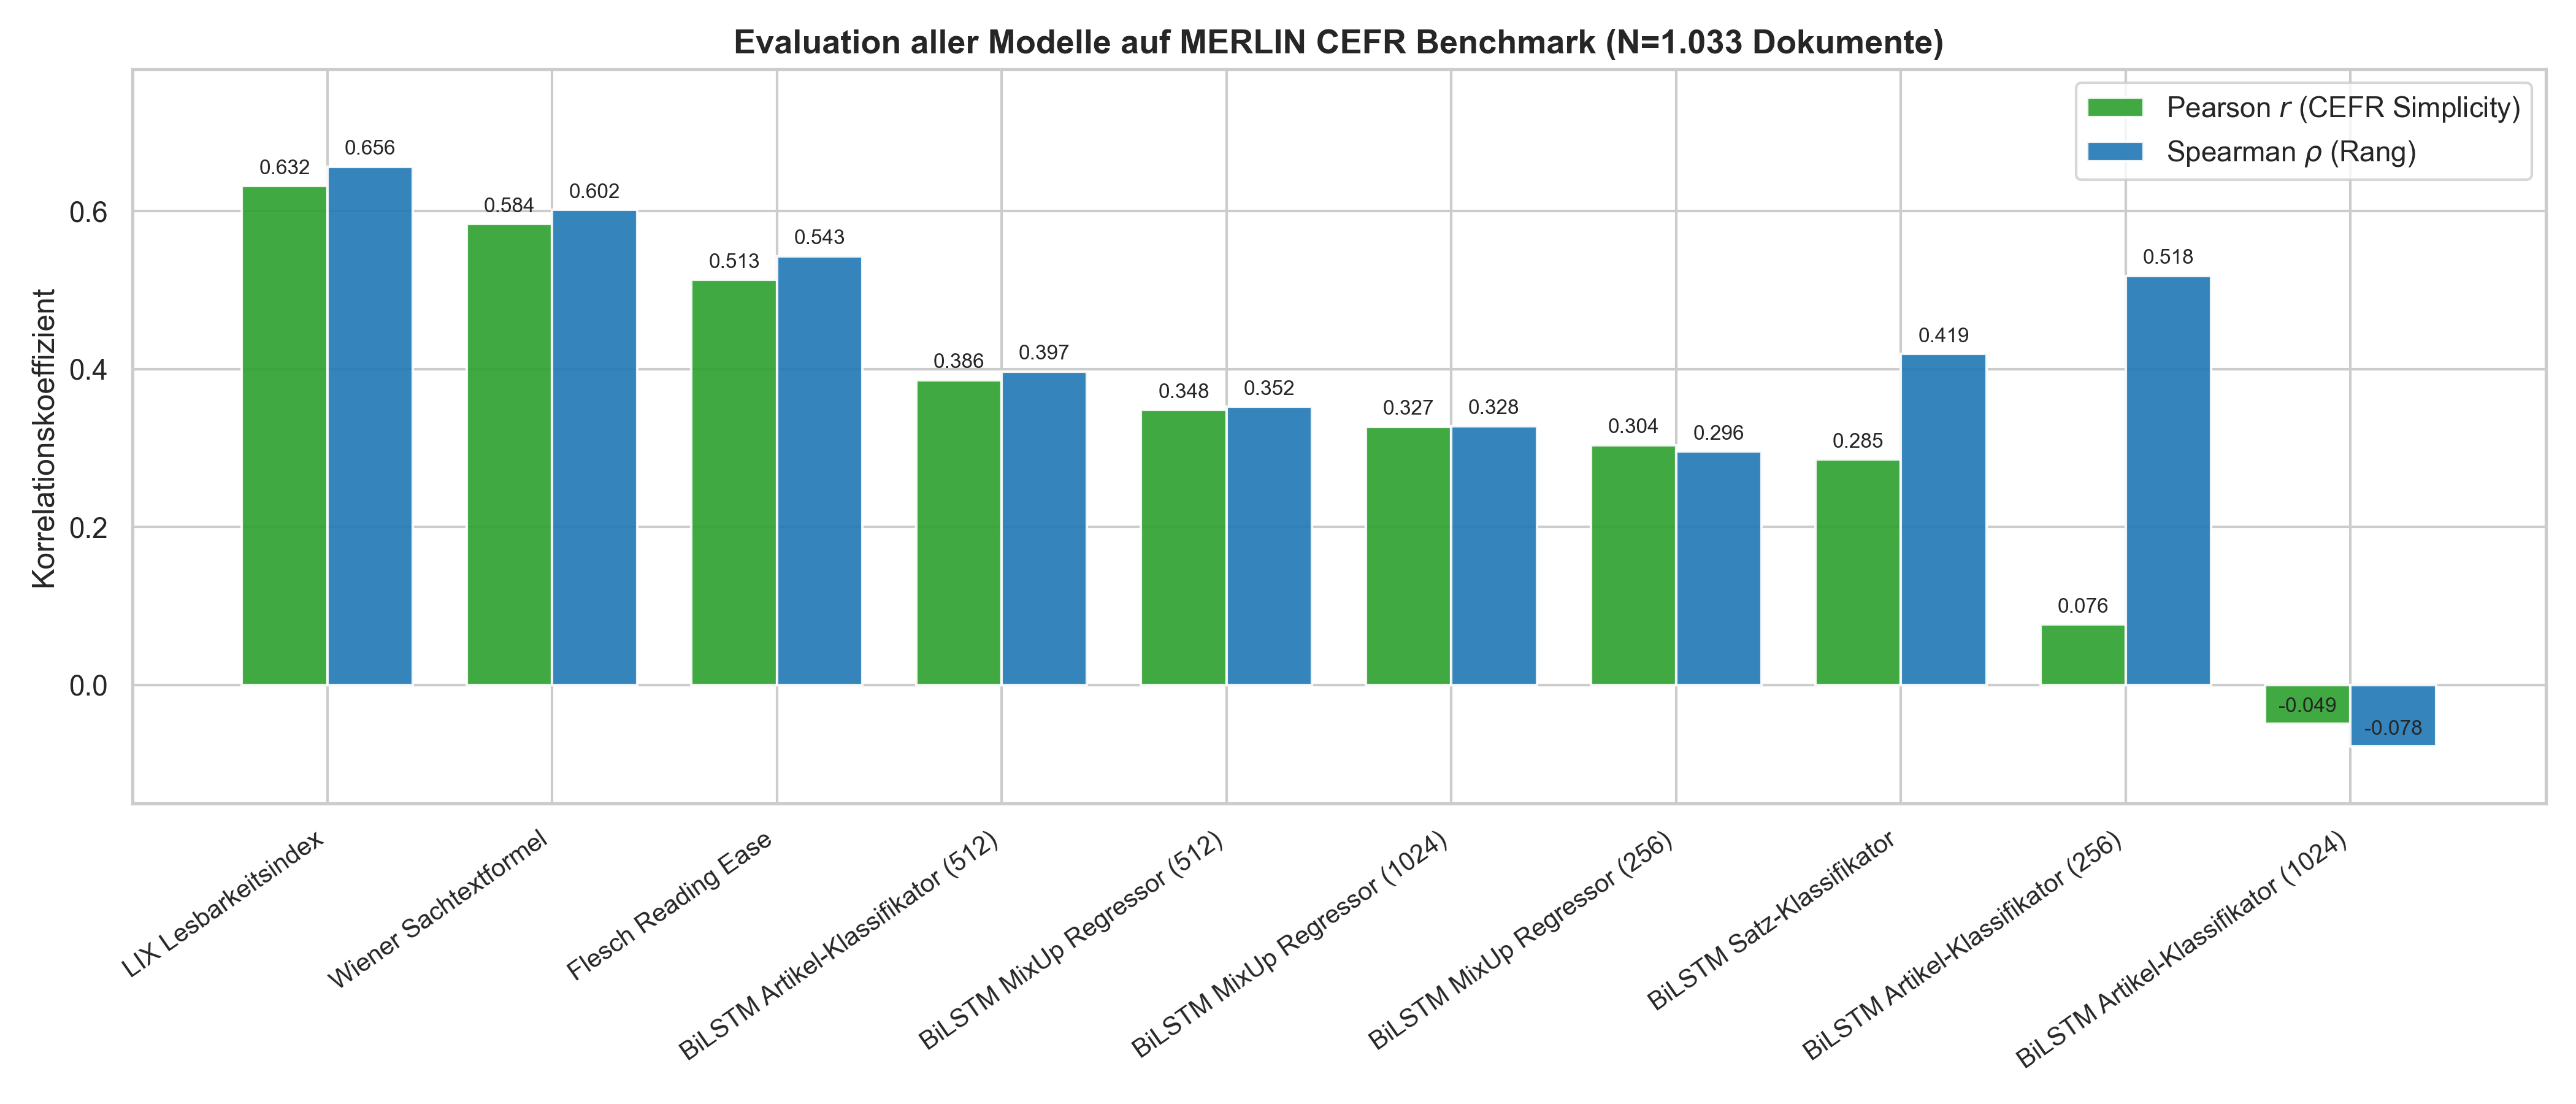
\includegraphics[width=0.95\textwidth]{images/merlin_correlation_barchart.png}
\caption{Pearson- und Spearman-Rangkorrelationen aller Modelle auf dem MERLIN CEFR-Benchmark ($N = 1.033$ Volltexte).}
\label{fig:anhang_merlin_barchart}
\end{figure}

\begin{figure}[htbp]
\centering

\includegraphics[width=\textwidth]{images/merlin_scatter_all_models_grid.png}
\caption{Streudiagramm-Grid aller 10 Modellvarianten gegen das kontinuierliche CEFR-Simplicity-Maß ($1{,}0 = \text{A1} \dots 0{,}0 = \text{C2}$) auf MERLIN inklusive Regressionsgeraden.}
\label{fig:anhang_merlin_scatter}
\end{figure}

\begin{figure}[htbp]
\centering

\includegraphics[width=\textwidth]{images/merlin_boxplots_all_models_grid.png}
\caption{Monotonie-Prüfung aller Modellfamilien: Boxplots der vorhergesagten Scores über die 5 CEFR-Stufen ($A1, A2, B1, B2, C1$) auf MERLIN (weiße Punkte kennzeichnen den Mittelwert).}
\label{fig:anhang_merlin_boxplots}
\end{figure}

\newpage
\subsection{Ergänzende Evaluation der Klassifikationsmodelle (In-Domain Sweet-Spot \& Granularitätsvergleich)}
\label{sec:anhang_klassifikatoren}

In diesem Abschnitt sind die ergänzenden empirischen Auswertungen zur binären Klassifikation dokumentiert: Tabelle~\ref{tab:sweet_spot_ablation_klassifikation} stellt die In-Domain-Klassifikationsgüte (Balanced Accuracy) über verschiedene Cosine-Similarity-Filterungsbereiche des internen Master-Korpus auf Satz- und Artikelebene gegenüber. Die Abbildungen~\ref{fig:anhang_classifier_kde} bis \ref{fig:anhang_classifier_confusion} visualisieren die Dichteverteilungen, ROC/PR-Kurven und Konfusionsmatrizen auf dem bereinigten \textit{Lebenshilfe}-Goldstandard ($N = 37$ Artikelpaare / $74$ Dokumente, $6.901$ Einzelsätze).

\begin{table}[htbp]
\centering
\small
\caption{In-Domain-Klassifikationsgüte (Balanced Accuracy) des BiLSTM in Abhängigkeit vom semantischen Similarity-Bereich und der Granularitätsebene auf dem internen Test-Split.}
\label{tab:sweet_spot_ablation_klassifikation}
\begin{tabular}{@{}lrrrr@{}}
\toprule
\textbf{Similarity-Bereich} & \shortstack[r]{\textbf{Artikelpaare}\\\textbf{(Anzahl)}} & \shortstack[r]{\textbf{Sätze}\\\textbf{(balanciert)}} & \shortstack[r]{\textbf{Satz-Level}\\\textbf{BAcc}} & \shortstack[r]{\textbf{Artikel-Level}\\\textbf{BAcc}} \\
\midrule
$0{,}60 \le \text{sim}_{\cos} \le 0{,}98$ & $1.474$ & $\sim 29.700$ & $92{,}48\,\%$ & $95{,}93\,\%$ \\
$0{,}70 \le \text{sim}_{\cos} \le 0{,}98$ & $1.362$ & $\sim 27.700$ & $92{,}43\,\%$ & $97{,}30\,\%$ \\
$\mathbf{0{,}80 \le \text{sim}_{\cos} \le 0{,}98}$ & $\mathbf{1.032}$ & $\mathbf{\sim 21.400}$ & $\mathbf{92{,}99\,\%}$ & $\mathbf{99{,}03\,\%}$ \\
$0{,}90 \le \text{sim}_{\cos} \le 0{,}98$ & $213$ & $\sim 4.800$ & $90{,}55\,\%$ & $98{,}44\,\%$ \\
\bottomrule
\end{tabular}
\end{table}

\begin{figure}[htbp]
\centering
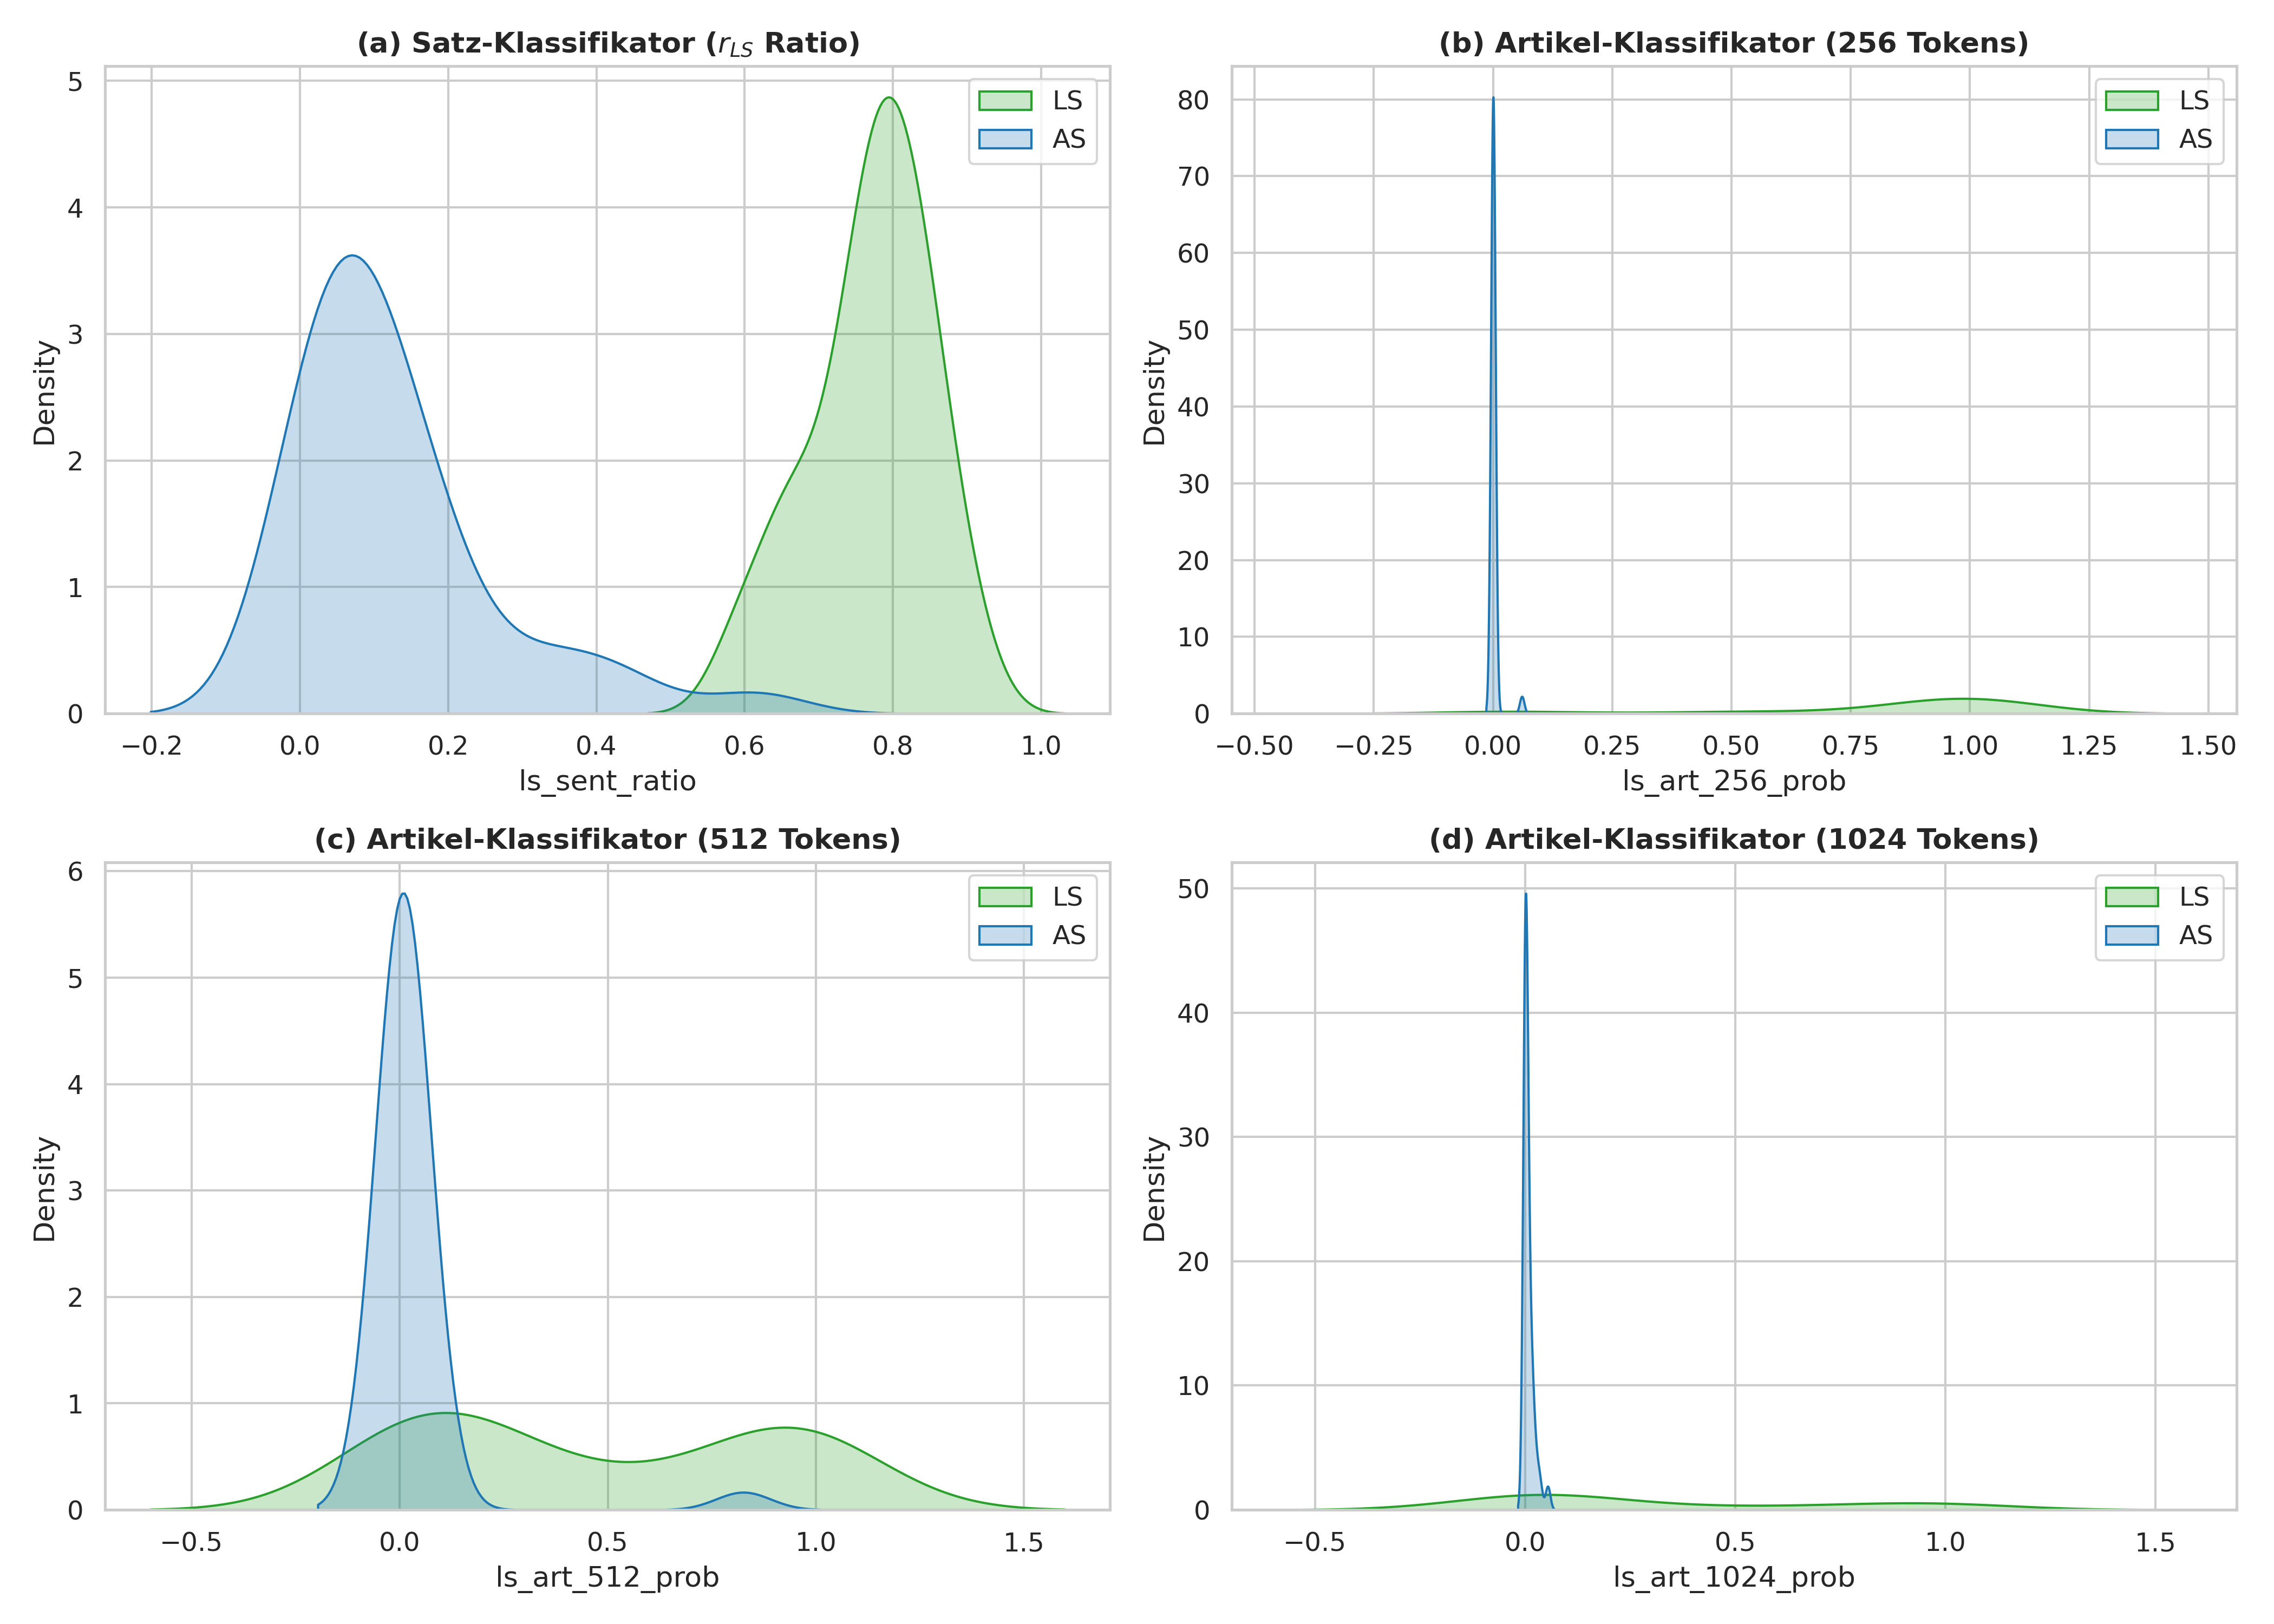
\includegraphics[width=0.95\textwidth]{images/classifier_kde_length_comparison.png}
\caption{Vergleich der Dichteverteilungen (KDE) für Leichte Sprache (LS, grün) und Alltagssprache (AS, blau) über alle Klassifikationsmodi: (a) BiLSTM Satz-Klassifikator (Simple-Sentence-Ratio $r_{LS}$), (b) BiLSTM Artikel-Klassifikator ($256$ Tokens), (c) BiLSTM Artikel-Klassifikator ($512$ Tokens) und (d) BiLSTM Artikel-Klassifikator ($1.024$ Tokens). Man beachte die ausgeprägte Asymmetrie: Während Alltagssprache durch scharfe Peaks bei $0{,}0$ überkonfident separiert wird, bricht die Konfidenz für Leichte Sprache bei längeren Artikelkontexten stark ein.}
\label{fig:anhang_classifier_kde}
\end{figure}

\begin{figure}[htbp]
\centering
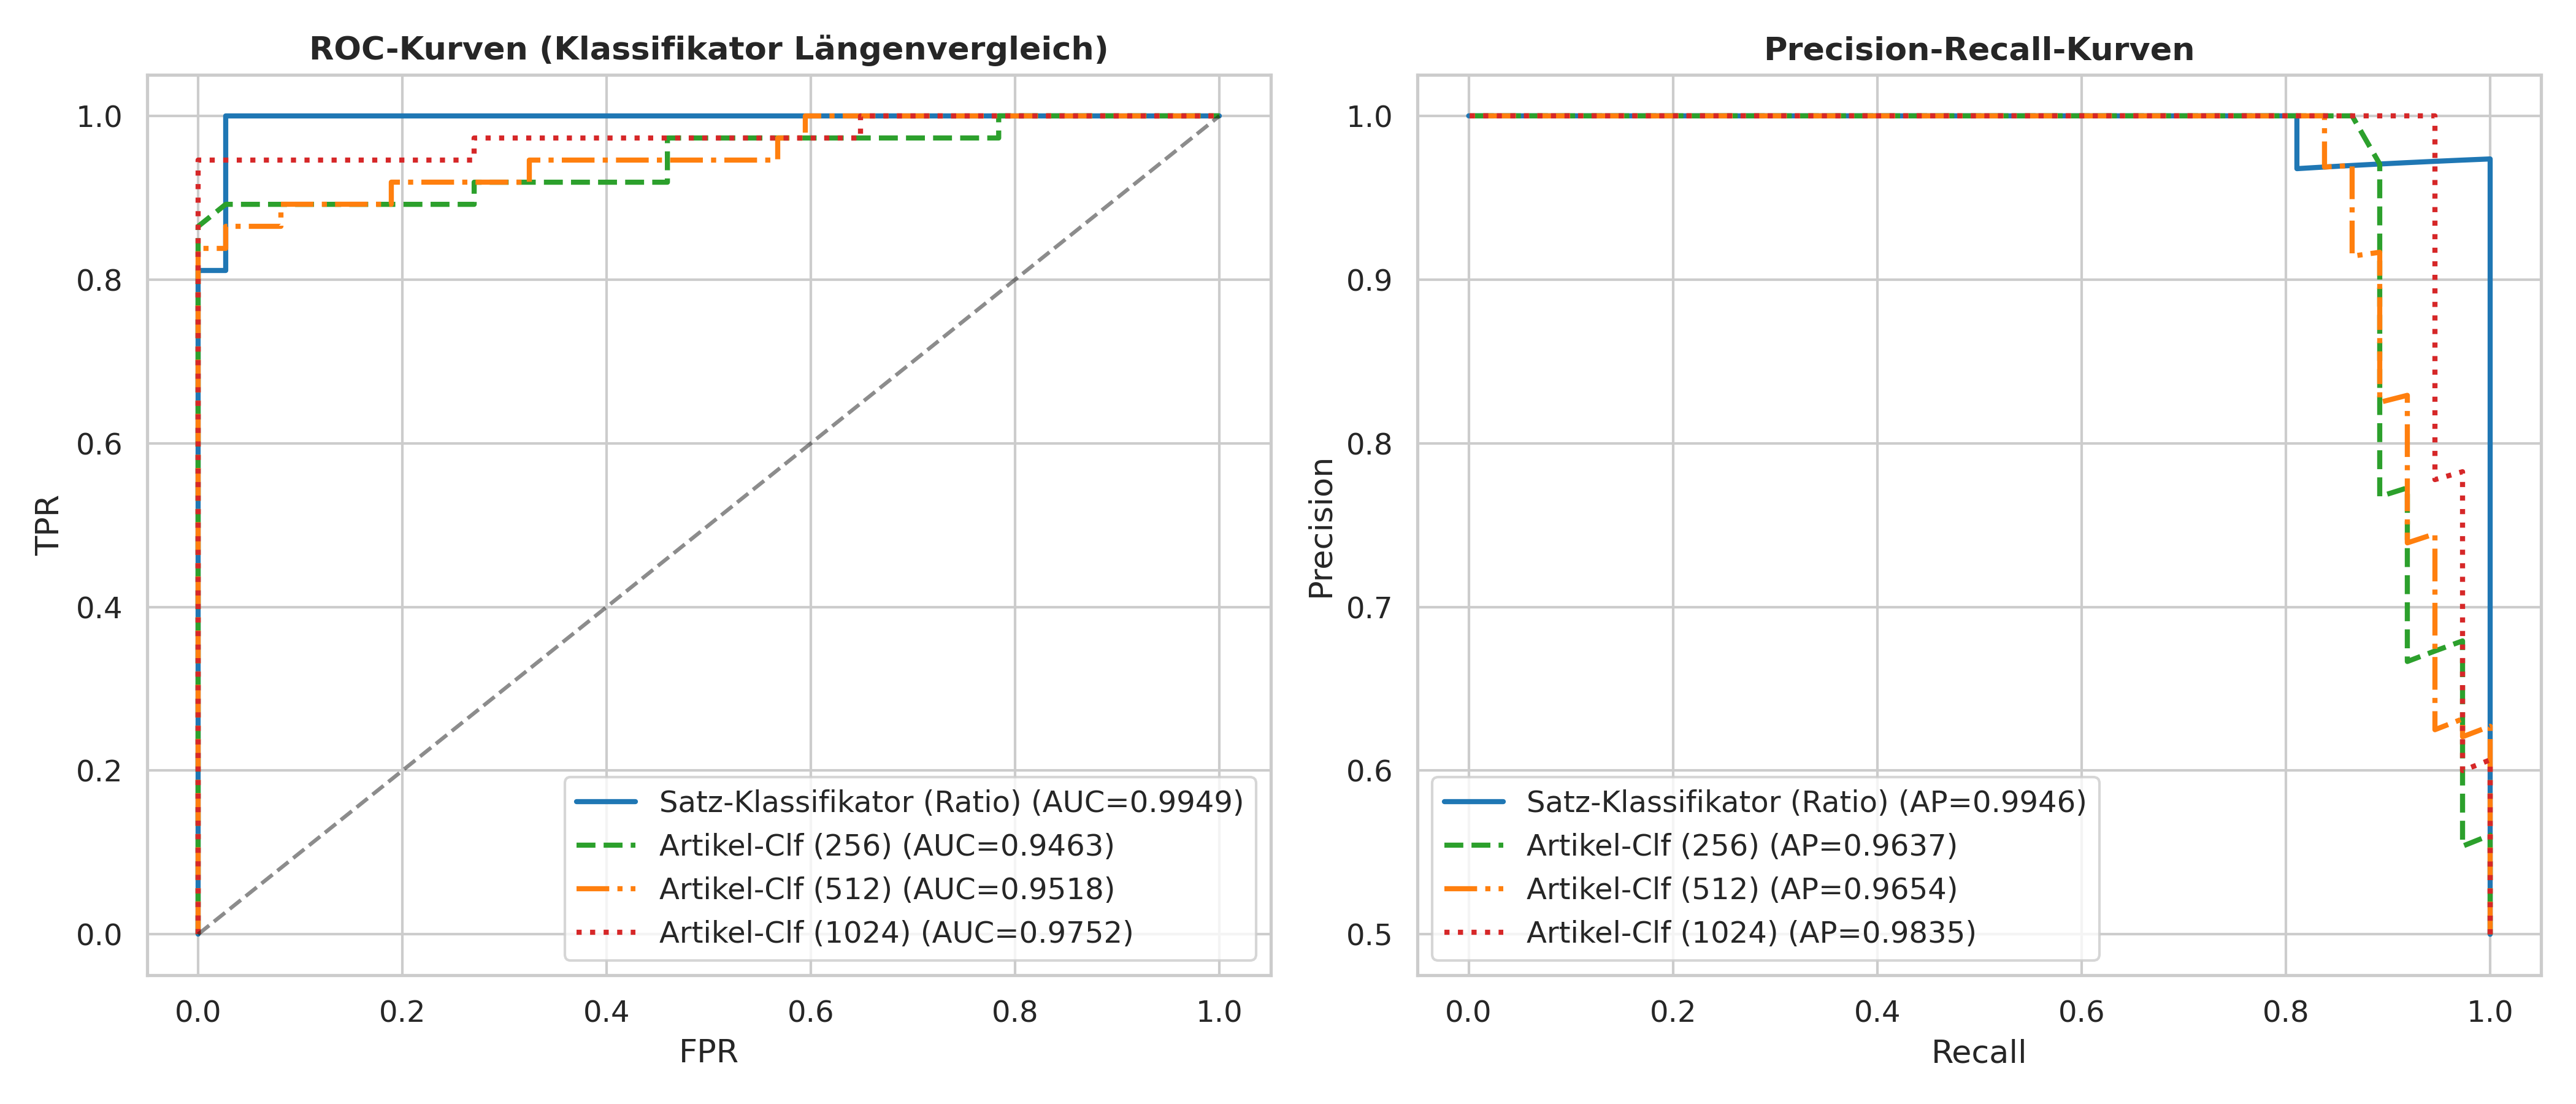
\includegraphics[width=0.95\textwidth]{images/classifier_roc_pr_length_comparison.png}
\caption{ROC- und Precision-Recall-Kurven der Klassifikationsmodelle auf dem Lebenshilfe-Goldstandard. Das Satzmodell mit Majority-Voting ($r_{LS}$) erzielt den höchsten AUC-Wert ($0{,}9985$) und übertrifft die direkten Artikelmodelle ($256$, $512$, $1.024$ Tokens) deutlich.}
\label{fig:anhang_classifier_roc_pr}
\end{figure}

\begin{figure}[htbp]
\centering

\includegraphics[width=\textwidth]{images/classifier_confusion_matrices.png}
\caption{Konfusionsmatrizen und relative Performanzmaße der Klassifikatoren: (1) Satz-Modell auf Einzelsatzebene ($N = 6.901$ Sätze), (2) Satz-Modell aggregiert via Majority Voting auf Dokumentebene ($N = 74$ Dokumente), (3) Artikel-Modell auf Dokumentebene sowie (4) vergleichende Gütekriterien im Balkendiagramm.}
\label{fig:anhang_classifier_confusion}
\end{figure}

\begin{table}[htbp]
\centering
\small
\caption{Multi-Seed-Stabilitäts-Benchmark aller Modellvarianten über $K=5$ Zufalls-Seeds ($42, 123, 456, 789, 1024$) auf dem Lebenshilfe-Goldstandard ($N = 37$ Artikelpaare / $74$ Dokumente).}
\label{tab:anhang_classifier_stability}
\adjustbox{max width=\textwidth}{%
\begin{tabular}{@{}lccccc@{}}
\toprule
\textbf{Modellarchitektur} & \textbf{Parameter} & \textbf{Balanced Acc ($\mu \pm \sigma$)} & \textbf{Min -- Max Spread} & \textbf{ROC-AUC ($\mu \pm \sigma$)} & \textbf{Pair Match ($\mu \pm \sigma$)} \\
\midrule
BiLSTM Satz-Klassifikator (MajVote)  & $3{,}46\text{ Mio.}$  & $\mathbf{97{,}03\,\% \pm 0{,}60\,\%}$ & $95{,}9\,\% - 97{,}3\,\%$ & $\mathbf{0{,}9966 \pm 0{,}0013}$ & $\mathbf{100{,}0\,\% \pm 0{,}0\,\%}$ \\
BiLSTM Artikel-1024 (Medium, $10k/64d$) & $\sim 700\text{ Tsd.}$ & $\mathbf{88{,}92\,\% \pm 3{,}75\,\%}$ & $83{,}8\,\% - 93{,}2\,\%$ & $0{,}9468 \pm 0{,}0342$ & $95{,}7\,\% \pm 3{,}1\,\%$ \\
BiLSTM Artikel-256 (Full, $25k/128d$) & $3{,}46\text{ Mio.}$  & $84{,}32\,\% \pm 8{,}47\,\%$ & $73{,}0\,\% - 93{,}2\,\%$ & $0{,}9675 \pm 0{,}0108$ & $96{,}8\,\% \pm 1{,}2\,\%$ \\
BiLSTM Artikel-512 (Full, $25k/128d$) & $3{,}46\text{ Mio.}$  & $82{,}16\,\% \pm 6{,}72\,\%$ & $71{,}6\,\% - 89{,}2\,\%$ & $0{,}9208 \pm 0{,}0329$ & $95{,}7\,\% \pm 2{,}4\,\%$ \\
BiLSTM Artikel-1024 (Tiny, $5k/32d$)  & $\sim 180\text{ Tsd.}$ & $81{,}62\,\% \pm 10{,}14\,\%$ & $73{,}0\,\% - 93{,}2\,\%$ & $0{,}9183 \pm 0{,}0443$ & $94{,}1\,\% \pm 4{,}0\,\%$ \\
BiLSTM Artikel-1024 (Full, $25k/128d$) & $3{,}46\text{ Mio.}$ & $\mathbf{80{,}00\,\% \pm 9{,}33\,\%}$ & $\mathbf{67{,}6\,\% - 91{,}9\,\%}$ & $0{,}9233 \pm 0{,}0485$ & $95{,}1\,\% \pm 5{,}2\,\%$ \\
\bottomrule
\end{tabular}}
\end{table}

\begin{figure}[htbp]
\centering
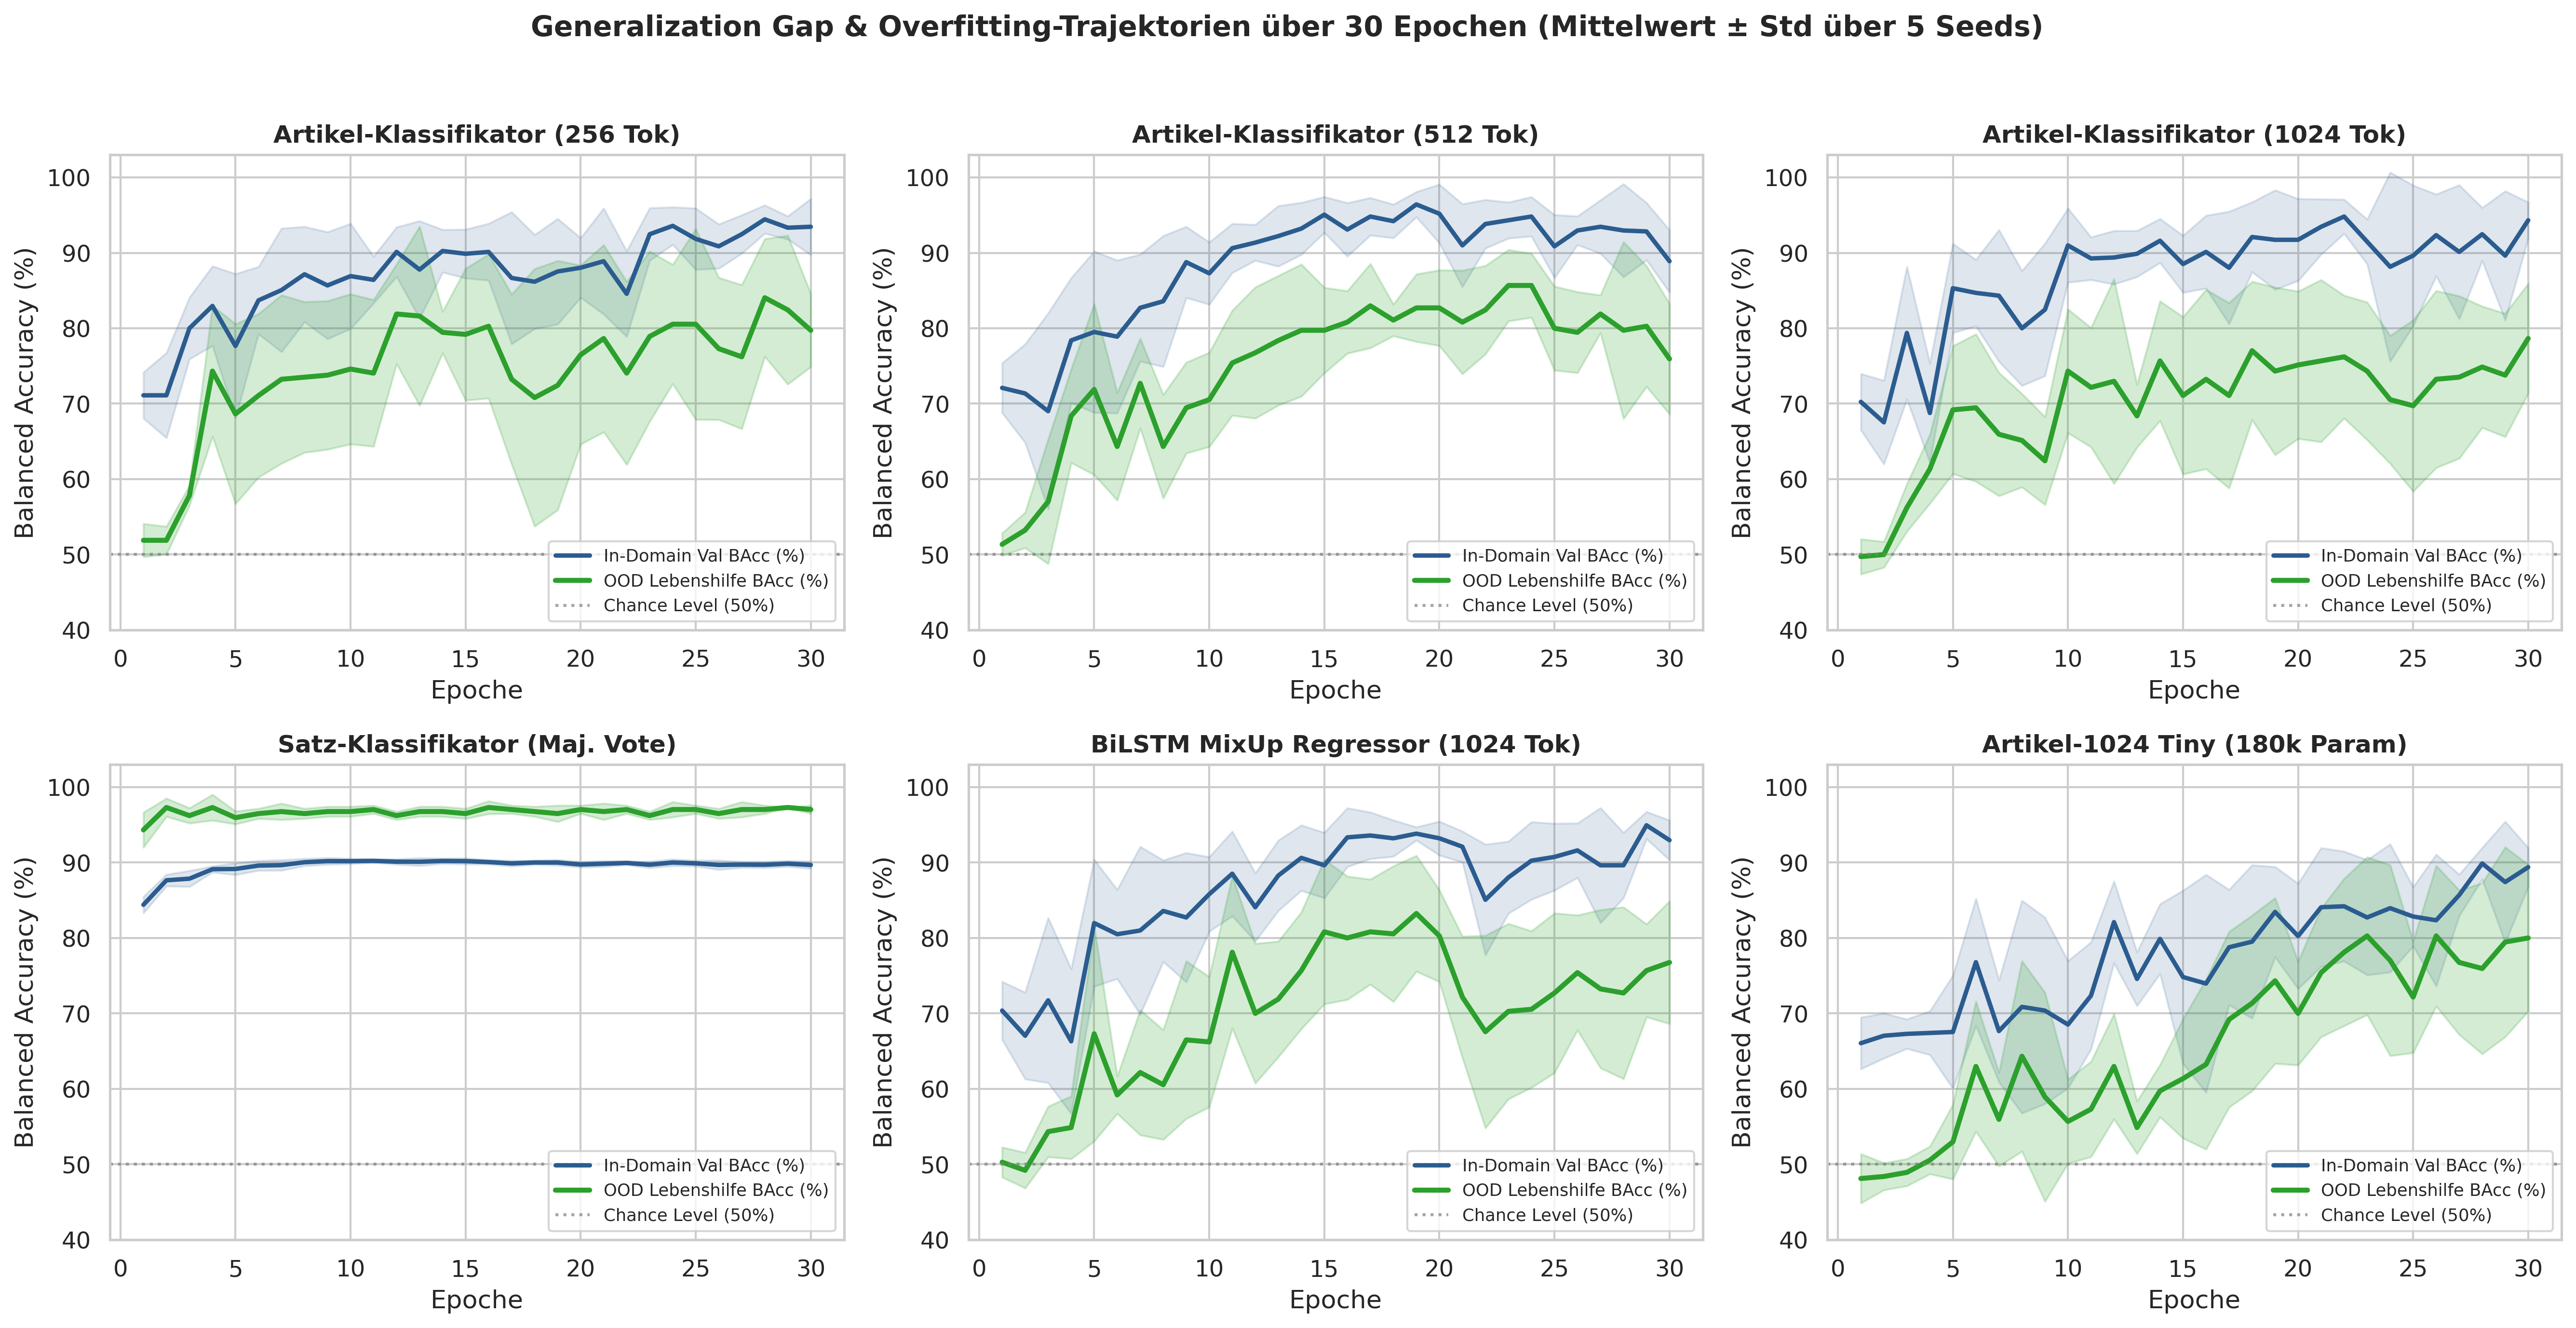
\includegraphics[width=0.95\textwidth]{images/generalization_gap_learning_curves.png}
\caption{Generalization Gap \& Overfitting-Trajektorien über 30 Epochen (Mittelwert $\pm$ Standardabweichung über 5 Seeds): Verlauf von In-Domain Validation Balanced Accuracy (blau) vs. Out-of-Domain Lebenshilfe Balanced Accuracy (grün).}
\label{fig:anhang_classifier_learning_curves}
\end{figure}

\begin{figure}[htbp]
\centering
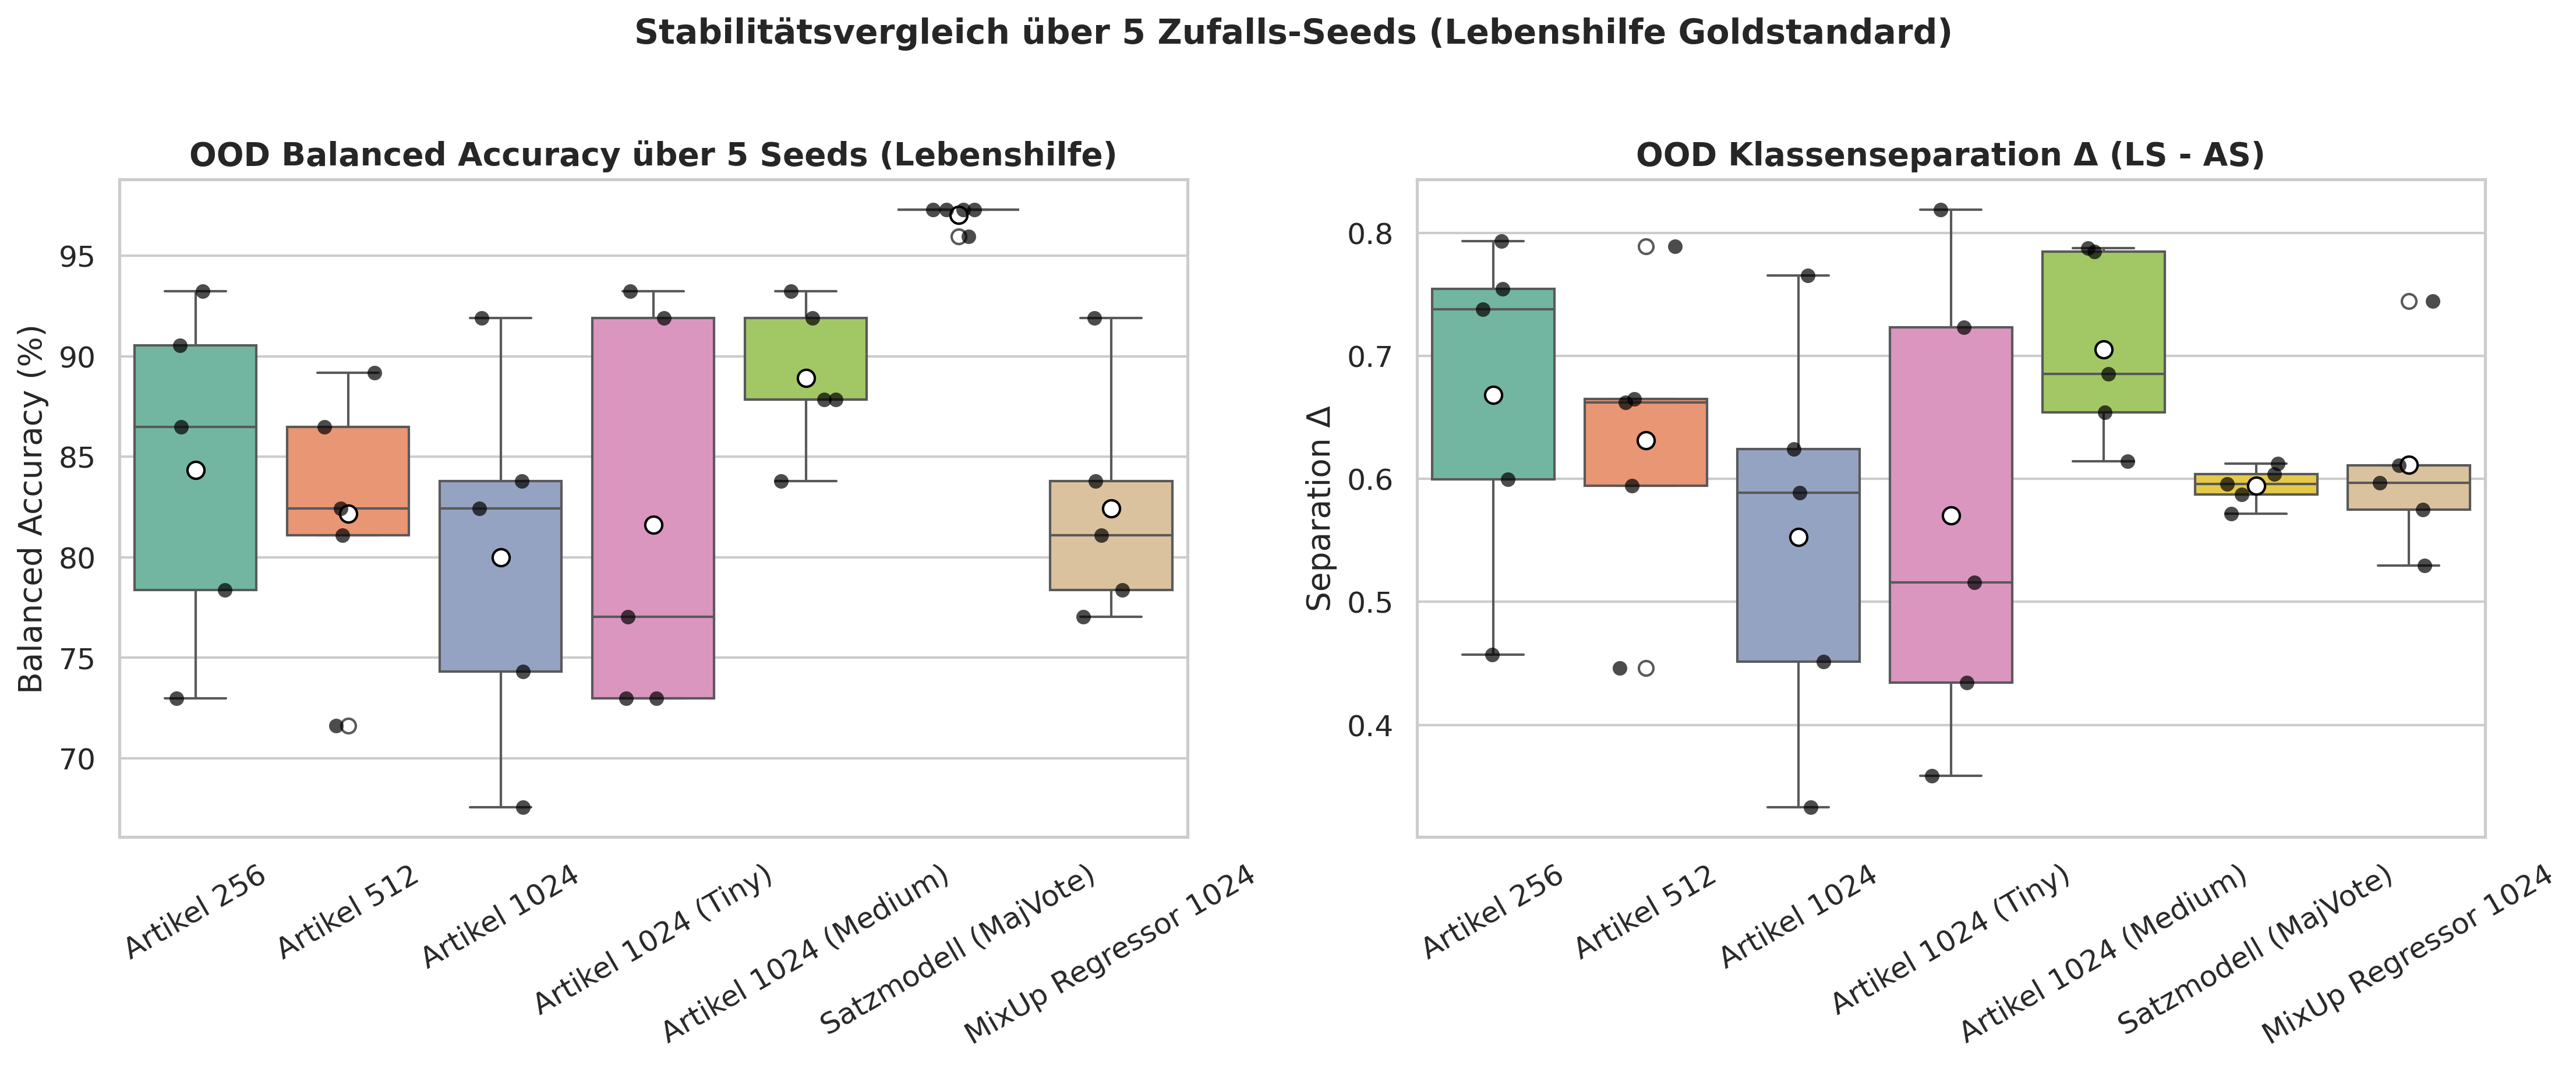
\includegraphics[width=0.95\textwidth]{images/multi_seed_boxplots.png}
\caption{Stabilitäts- und Varianzvergleich über 5 Zufalls-Seeds auf dem Lebenshilfe-Goldstandard: Boxplots von Balanced Accuracy (\%) und Klassenseparation $\Delta$ für alle Modellkonfigurationen.}
\label{fig:anhang_classifier_boxplots}
\end{figure}

\newpage
\subsection{Ergänzende Evaluation der MixUp Trainings- und Sampling-Strategien (Varianten A--D)}
\label{sec:anhang_mixup_varianten}

In diesem Abschnitt sind die empirischen Benchmark-Ergebnisse und grafischen Analysen zu den vier untersuchten Dataloader- und Optimierungsstrategien des kontinuierlichen BiLSTM MixUp-Regressors dokumentiert:
\begin{itemize}
    \item \textbf{Variante A (Statisch):} Feste Vorabmischung und Shuffling bei der Initialisierung des Datasets ($p_{\text{dynamic}} = 0{,}0$).
    \item \textbf{Variante B (Dynamisch):} Rein dynamisches On-the-Fly-Mischen und Shuffling pro Batch ($p_{\text{dynamic}} = 1{,}0$).
    \item \textbf{Variante C (Hybrid):} Epochenabhängiges Curriculum-Mischen mit linear ansteigendem Dynamic-Anteil ($p_{\text{dynamic}} = \frac{\text{Epoche}}{\text{Gesamtepochen}}$).
    \item \textbf{Variante D (Hybrid + Cyclic LR):} Hybrid-Mischung kombiniert mit zyklischem Lernratenscheduling mittels \textit{CosineAnnealingWarmRestarts}.
\end{itemize}

Tabelle~\ref{tab:anhang_mixup_varianten_benchmark} stellt die Gütemaße auf dem internen Test-Split (In-Domain, $N = 2.968$ Sätze / $2.560$ Mischungen) und dem externen \textit{Lebenshilfe}-Goldstandard (Out-of-Domain, $N = 2.236$ Sätze / $1.476$ Mischungen) gegenüber. Die Abbildungen~\ref{fig:anhang_mixup_variants_kde} und \ref{fig:anhang_mixup_variants_scatter} visualisieren die resultierenden Dichteverteilungen und Regressions-Trajektorien auf dem Lebenshilfe-Datensatz.

\begin{table}[htbp]
\centering
\small
\caption{Gesamtevaluation der vier MixUp-Trainings- und Sampling-Strategien auf dem internen Test-Split (In-Domain) und dem Lebenshilfe-Goldstandard (Out-of-Domain).}
\label{tab:anhang_mixup_varianten_benchmark}
\adjustbox{max width=\textwidth}{%
\begin{tabular}{@{}lcccccccccc@{}}
\toprule
 & \multicolumn{5}{c}{\textbf{In-Domain Test-Split}} & \multicolumn{5}{c}{\textbf{Out-of-Domain Lebenshilfe}} \\
\cmidrule(lr){2-6} \cmidrule(lr){7-11}
\textbf{Sampling-Strategie} & \textbf{\O{} $\lambda$ (LS)} & \textbf{\O{} $\lambda$ (AS)} & \textbf{BAcc} & \textbf{Reg-MSE} & \textbf{Reg-MAE} & \textbf{\O{} $\lambda$ (LS)} & \textbf{\O{} $\lambda$ (AS)} & \textbf{BAcc} & \textbf{Reg-MSE} & \textbf{Reg-MAE} \\
\midrule
Variante A (Statisch)          & $0{,}793$ & $0{,}090$ & $\mathbf{95{,}71\,\%}$ & $0{,}0274$ & $0{,}1238$ & $\mathbf{0{,}738}$ & $0{,}094$ & $\mathbf{94{,}50\,\%}$ & $\mathbf{0{,}0421}$ & $\mathbf{0{,}1569}$ \\
Variante B (Dynamisch)         & $0{,}788$ & $0{,}085$ & $95{,}07\,\%$ & $\mathbf{0{,}0263}$ & $\mathbf{0{,}1192}$ & $0{,}680$ & $0{,}089$ & $91{,}37\,\%$ & $0{,}0528$ & $0{,}1771$ \\
Variante C (Hybrid)            & $\mathbf{0{,}807}$ & $0{,}095$ & $95{,}23\,\%$ & $0{,}0279$ & $0{,}1254$ & $0{,}710$ & $0{,}097$ & $91{,}18\,\%$ & $0{,}0468$ & $0{,}1672$ \\
Variante D (Hybrid + Cyclic LR)& $0{,}802$ & $\mathbf{0{,}075}$ & $95{,}55\,\%$ & $0{,}0274$ & $0{,}1233$ & $0{,}714$ & $\mathbf{0{,}078}$ & $91{,}71\,\%$ & $0{,}0486$ & $0{,}1710$ \\
\bottomrule
\end{tabular}}
\end{table}

\begin{figure}[htbp]
\centering
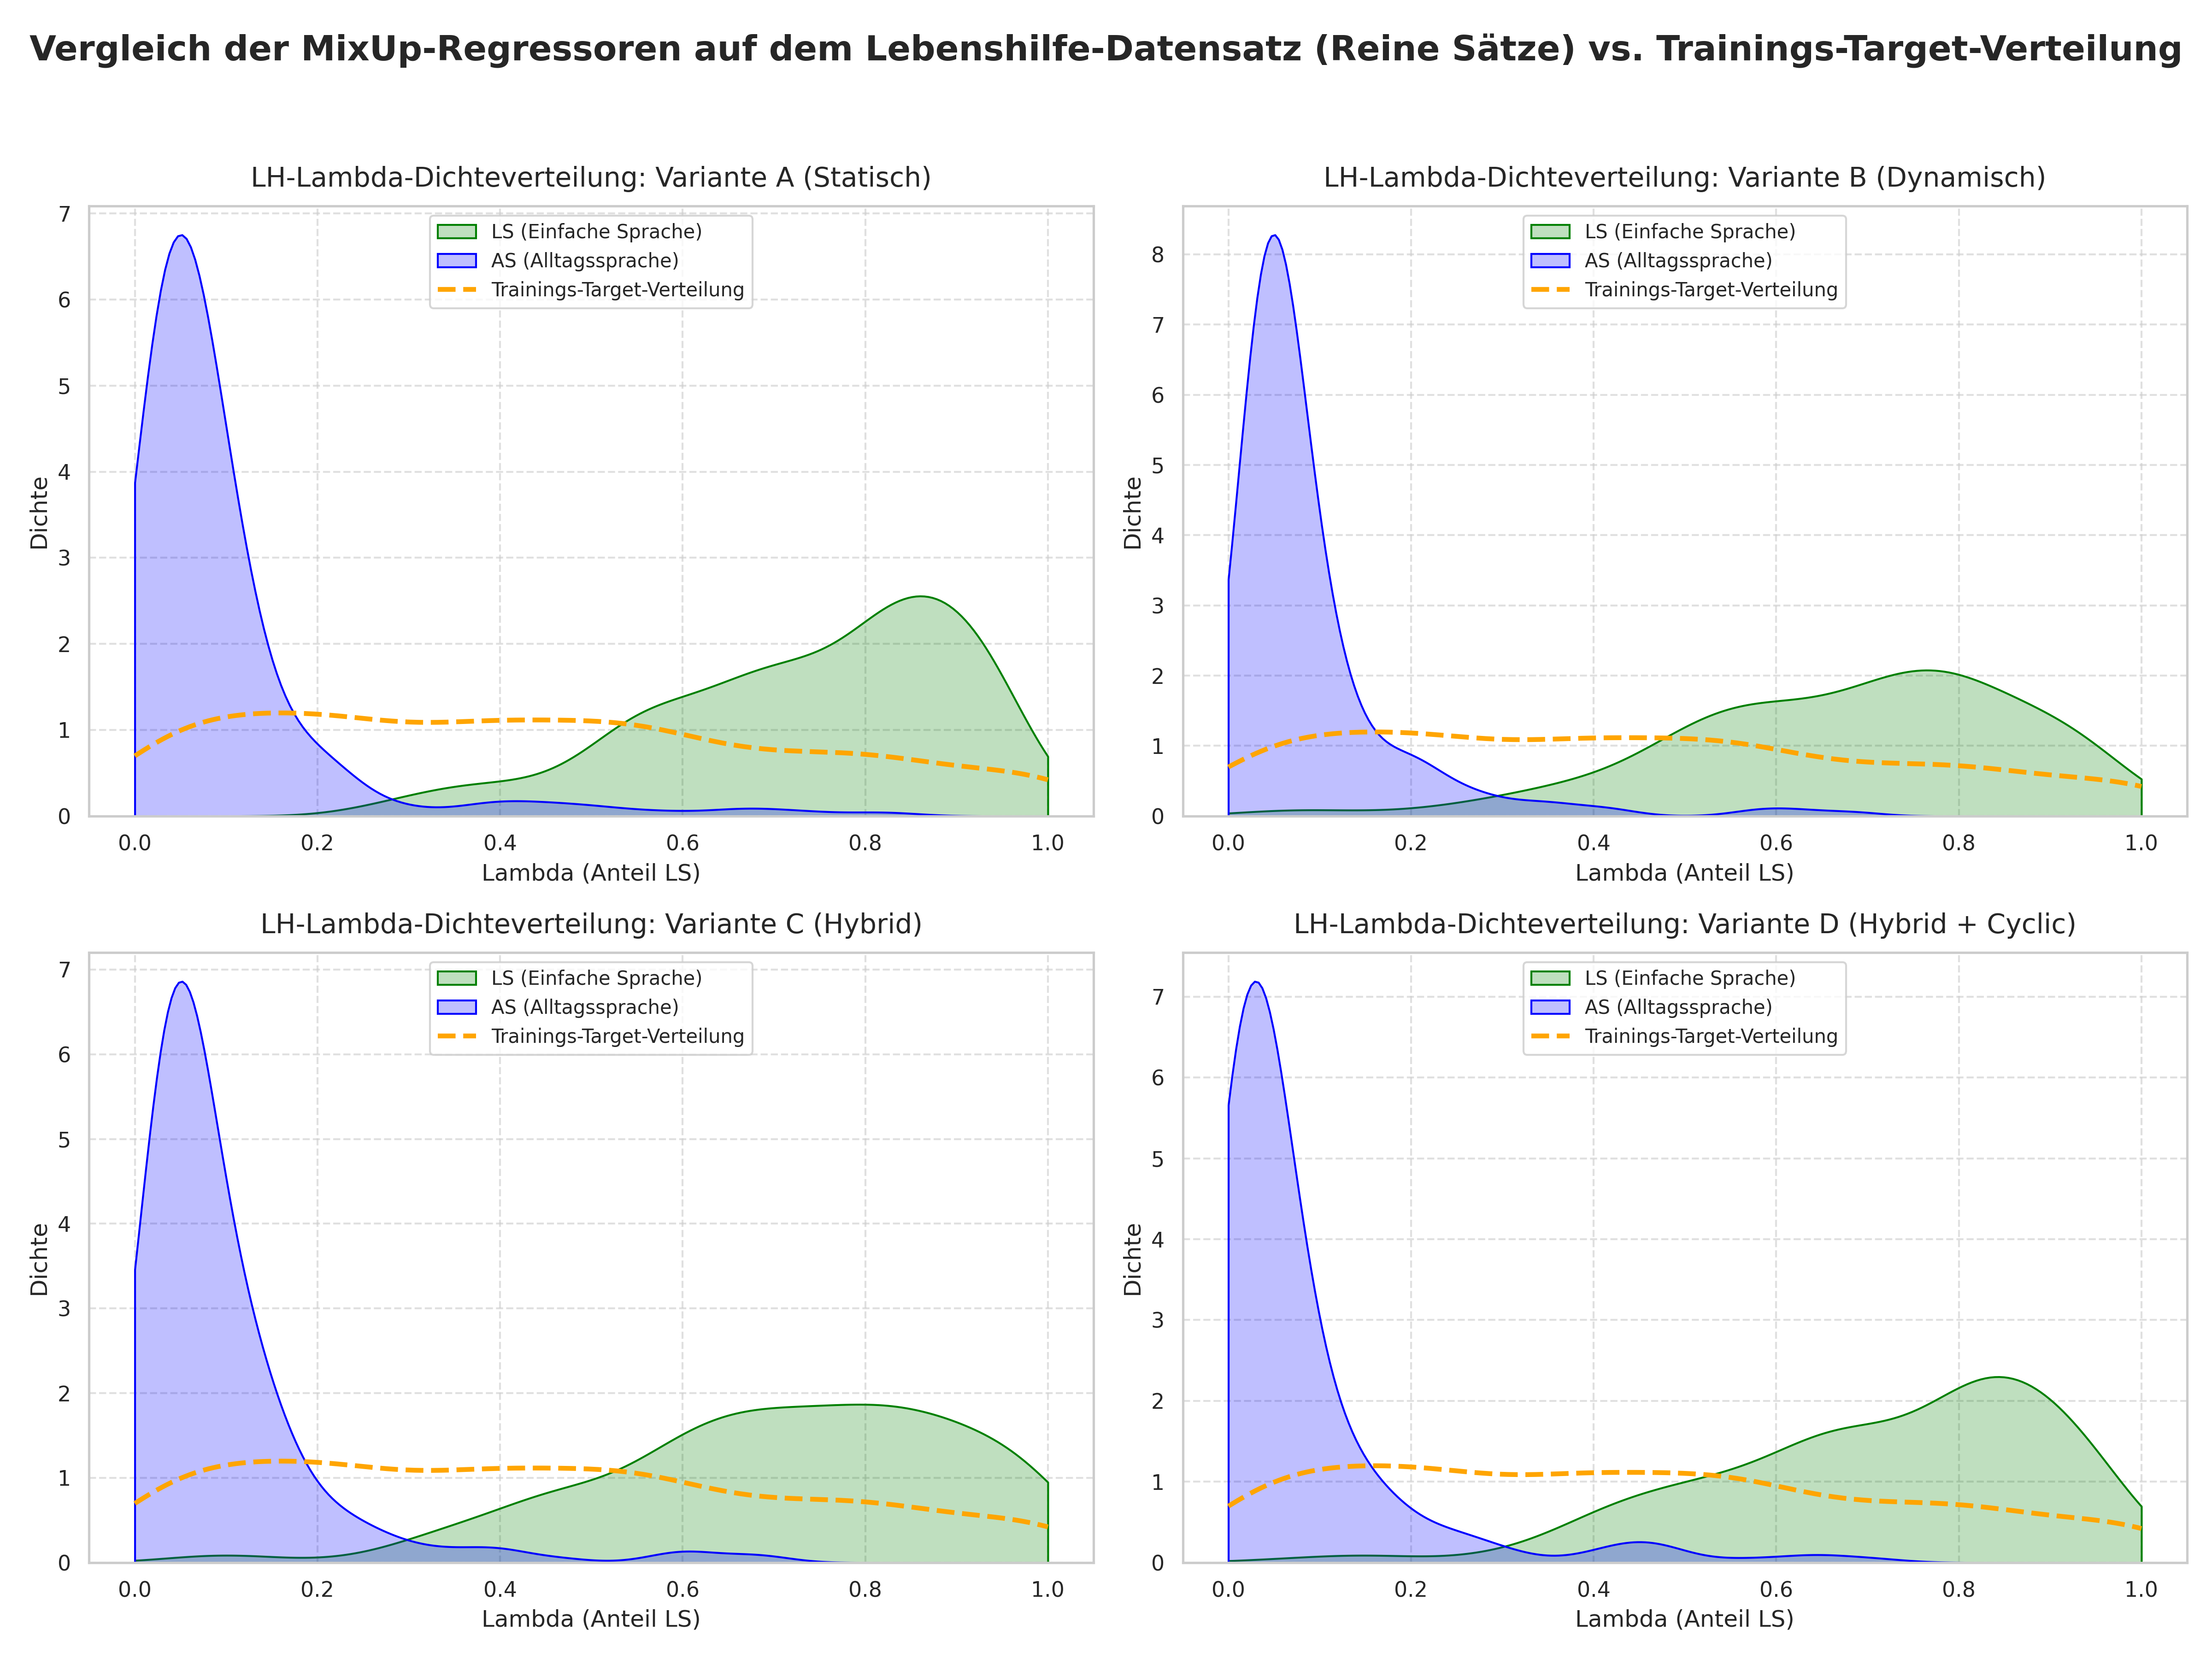
\includegraphics[width=\textwidth]{images/mixup_variants_lh_kde.png}
\caption{KDE-Dichteverteilungen der vorhergesagten Scores für reine Alltagssprache (AS, blau) und reine Leichte Sprache (LS, grün) auf dem Lebenshilfe-Goldstandard im Vergleich zur Zielverteilung im Training (gestrichelte Kurve) für die vier Sampling-Strategien (Varianten A bis D).}
\label{fig:anhang_mixup_variants_kde}
\end{figure}

\begin{figure}[htbp]
\centering
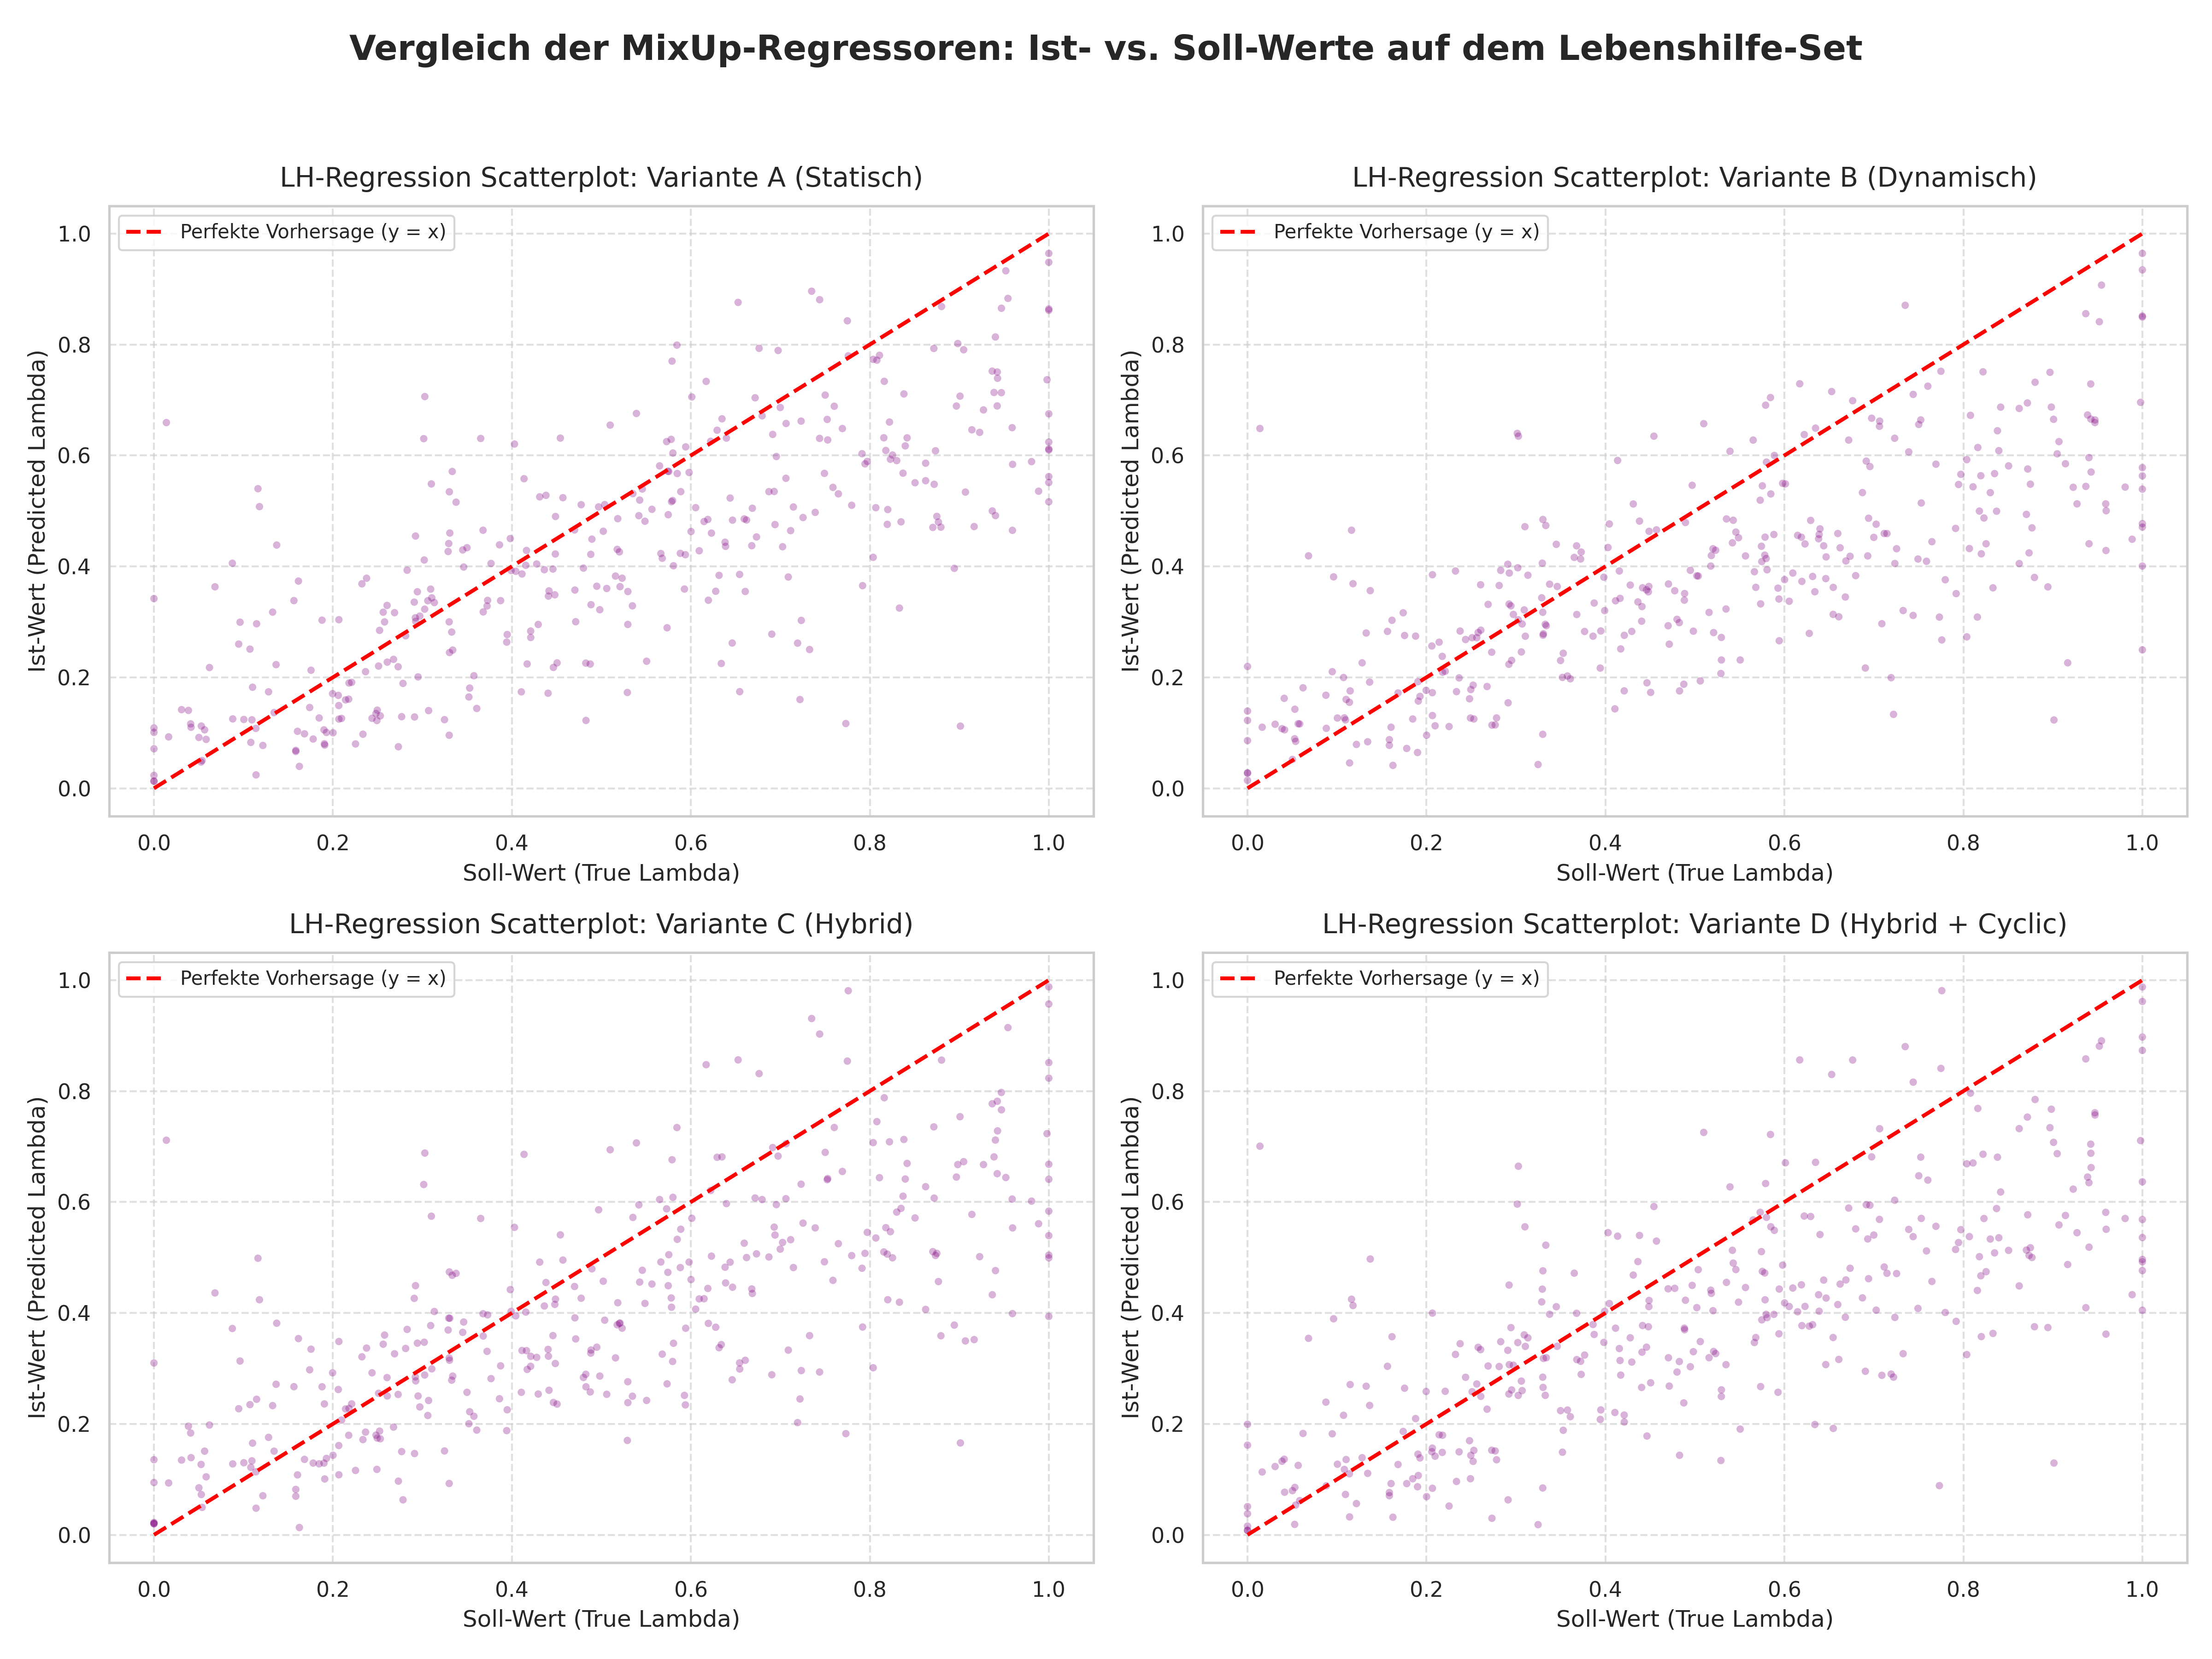
\includegraphics[width=\textwidth]{images/mixup_variants_lh_scatter.png}
\caption{Streudiagramme der Regressionsvorhersagen $\hat{\lambda}$ auf dem Lebenshilfe-Goldstandard: Wahre kontinuierliche Zielwerte $\lambda \in [0{,}0, 1{,}0]$ auf der x-Achse gegen Modellvorhersagen auf der y-Achse inklusive linearer Regressionsgerade (rot) und idealer Diagonalen (gestrichelt) über alle vier Modellvarianten.}
\label{fig:anhang_mixup_variants_scatter}
\end{figure}

\newpage
\subsection{Ergänzende Evaluation der BiLSTM MixUp Regressoren (Längenvergleich \& Trajektorien)}
\label{sec:anhang_regressoren_laengen}

In diesem Abschnitt sind die ergänzenden grafischen Auswertungen zur Kontextlängen-Ablation der kontinuierlichen BiLSTM MixUp Regressoren ($256$, $512$ und $1.024$ Tokens) auf dem \textit{Lebenshilfe}-Goldstandard dargestellt.

\begin{figure}[htbp]
\centering
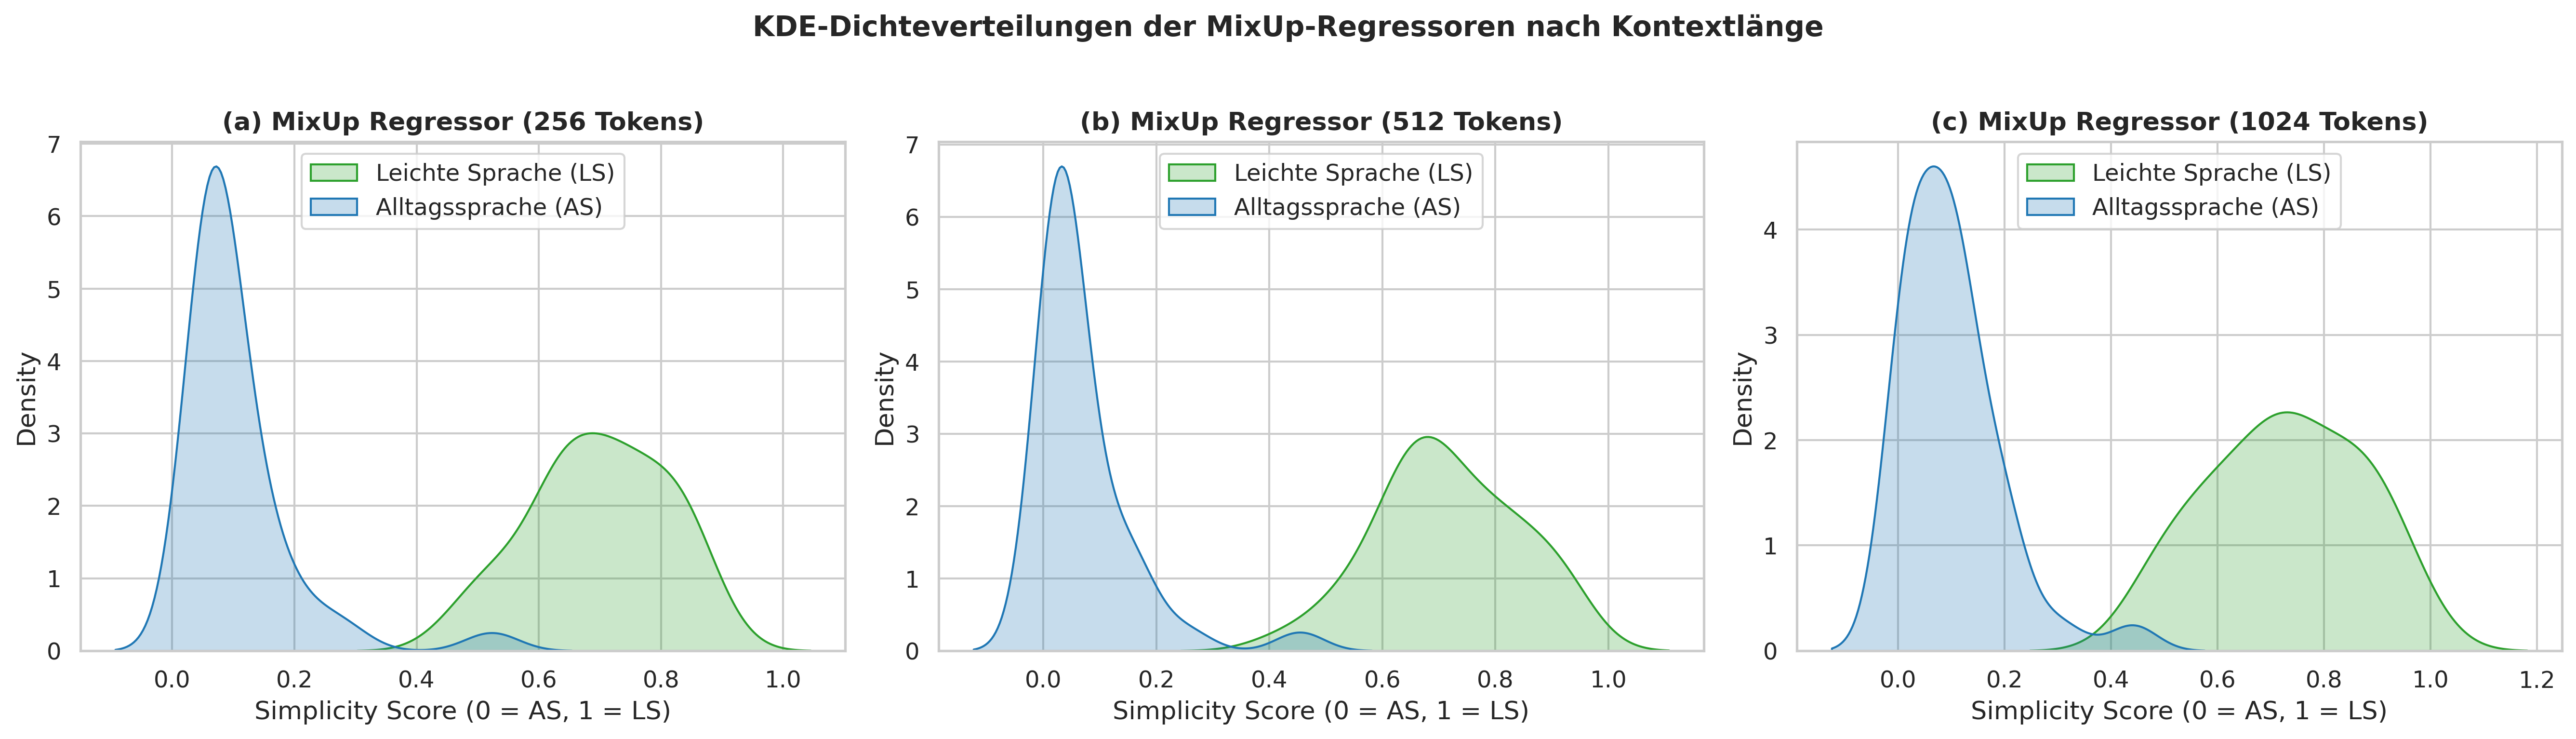
\includegraphics[width=0.95\textwidth]{images/regressor_kde_length_comparison.png}
\caption{KDE-Dichteverteilungen der BiLSTM MixUp Regressoren für Leichte Sprache (LS, grün) und Alltagssprache (AS, blau) über verschiedene Kontextlängen: (a) $256$ Tokens, (b) $512$ Tokens und (c) $1.024$ Tokens. Im Gegensatz zum binären Klassifikator weisen die Regressoren bei allen Längen wohlgeformte, breit separierte Verteilungen auf, wobei das $1.024$-Token-Modell die geringste Varianz und schärfste Trennung erzielt.}
\label{fig:anhang_regressor_kde}
\end{figure}

\begin{figure}[htbp]
\centering
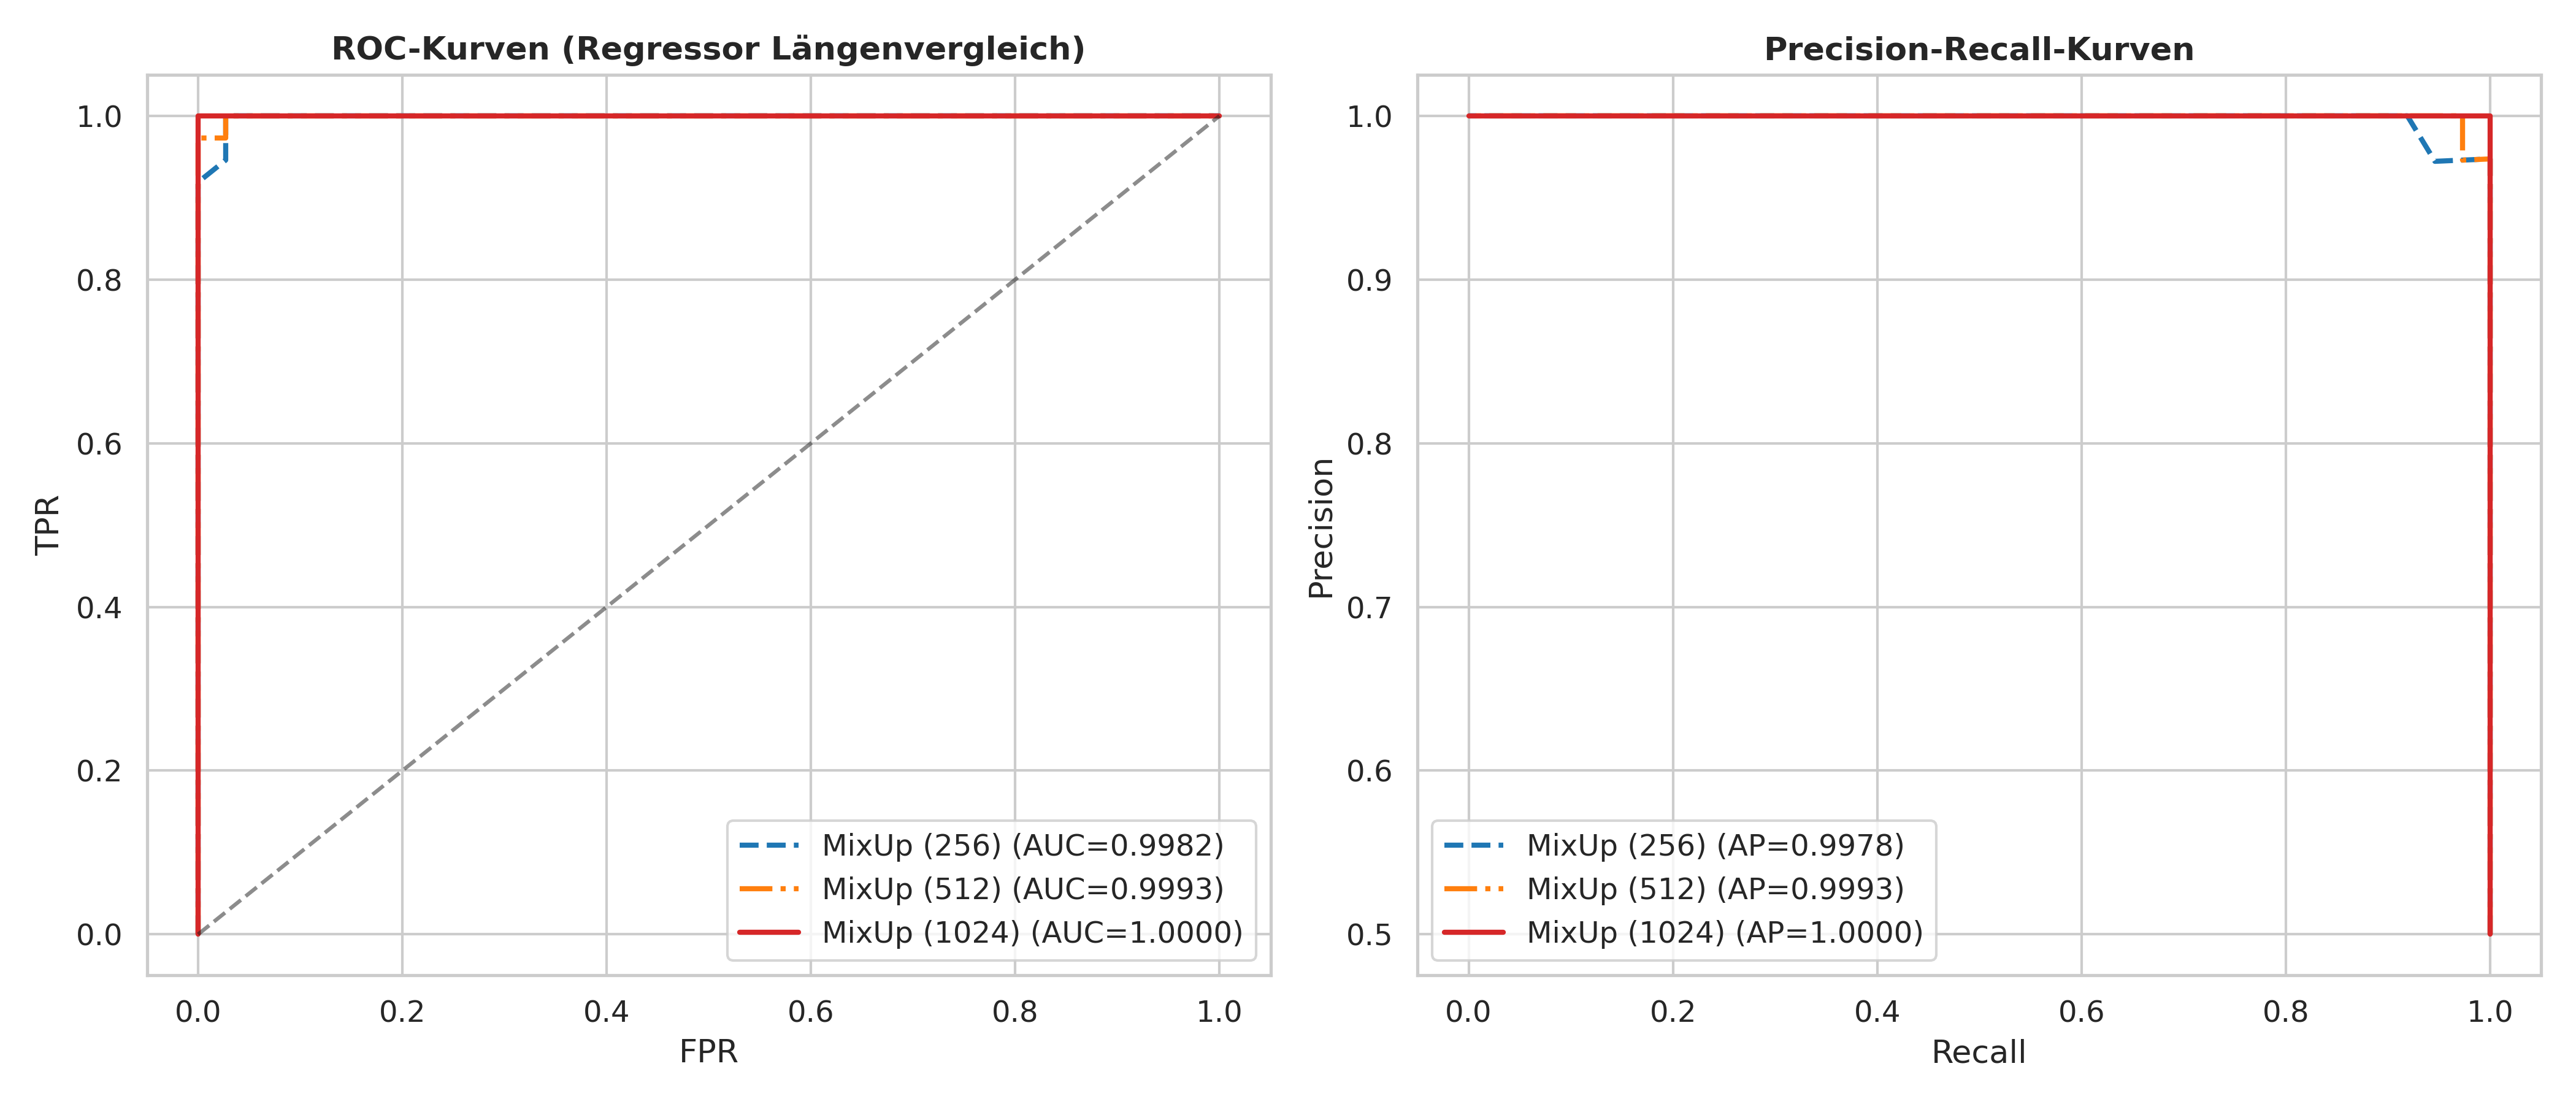
\includegraphics[width=0.95\textwidth]{images/regressor_roc_pr_length_comparison.png}
\caption{ROC- und Precision-Recall-Kurven der BiLSTM MixUp Regressoren ($256$, $512$, $1.024$ Tokens) auf dem Lebenshilfe-Goldstandard. Alle drei Varianten erreichen herausragende Diskriminationswerte ($\text{ROC-AUC} \ge 0{,}998$, $\text{PR-AUC} \ge 0{,}997$), wobei die $1.024$-Token-Konfiguration mit $\text{ROC-AUC} = 0{,}9993$ dominiert.}
\label{fig:anhang_regressor_roc_pr}
\end{figure}

\begin{figure}[htbp]
\centering
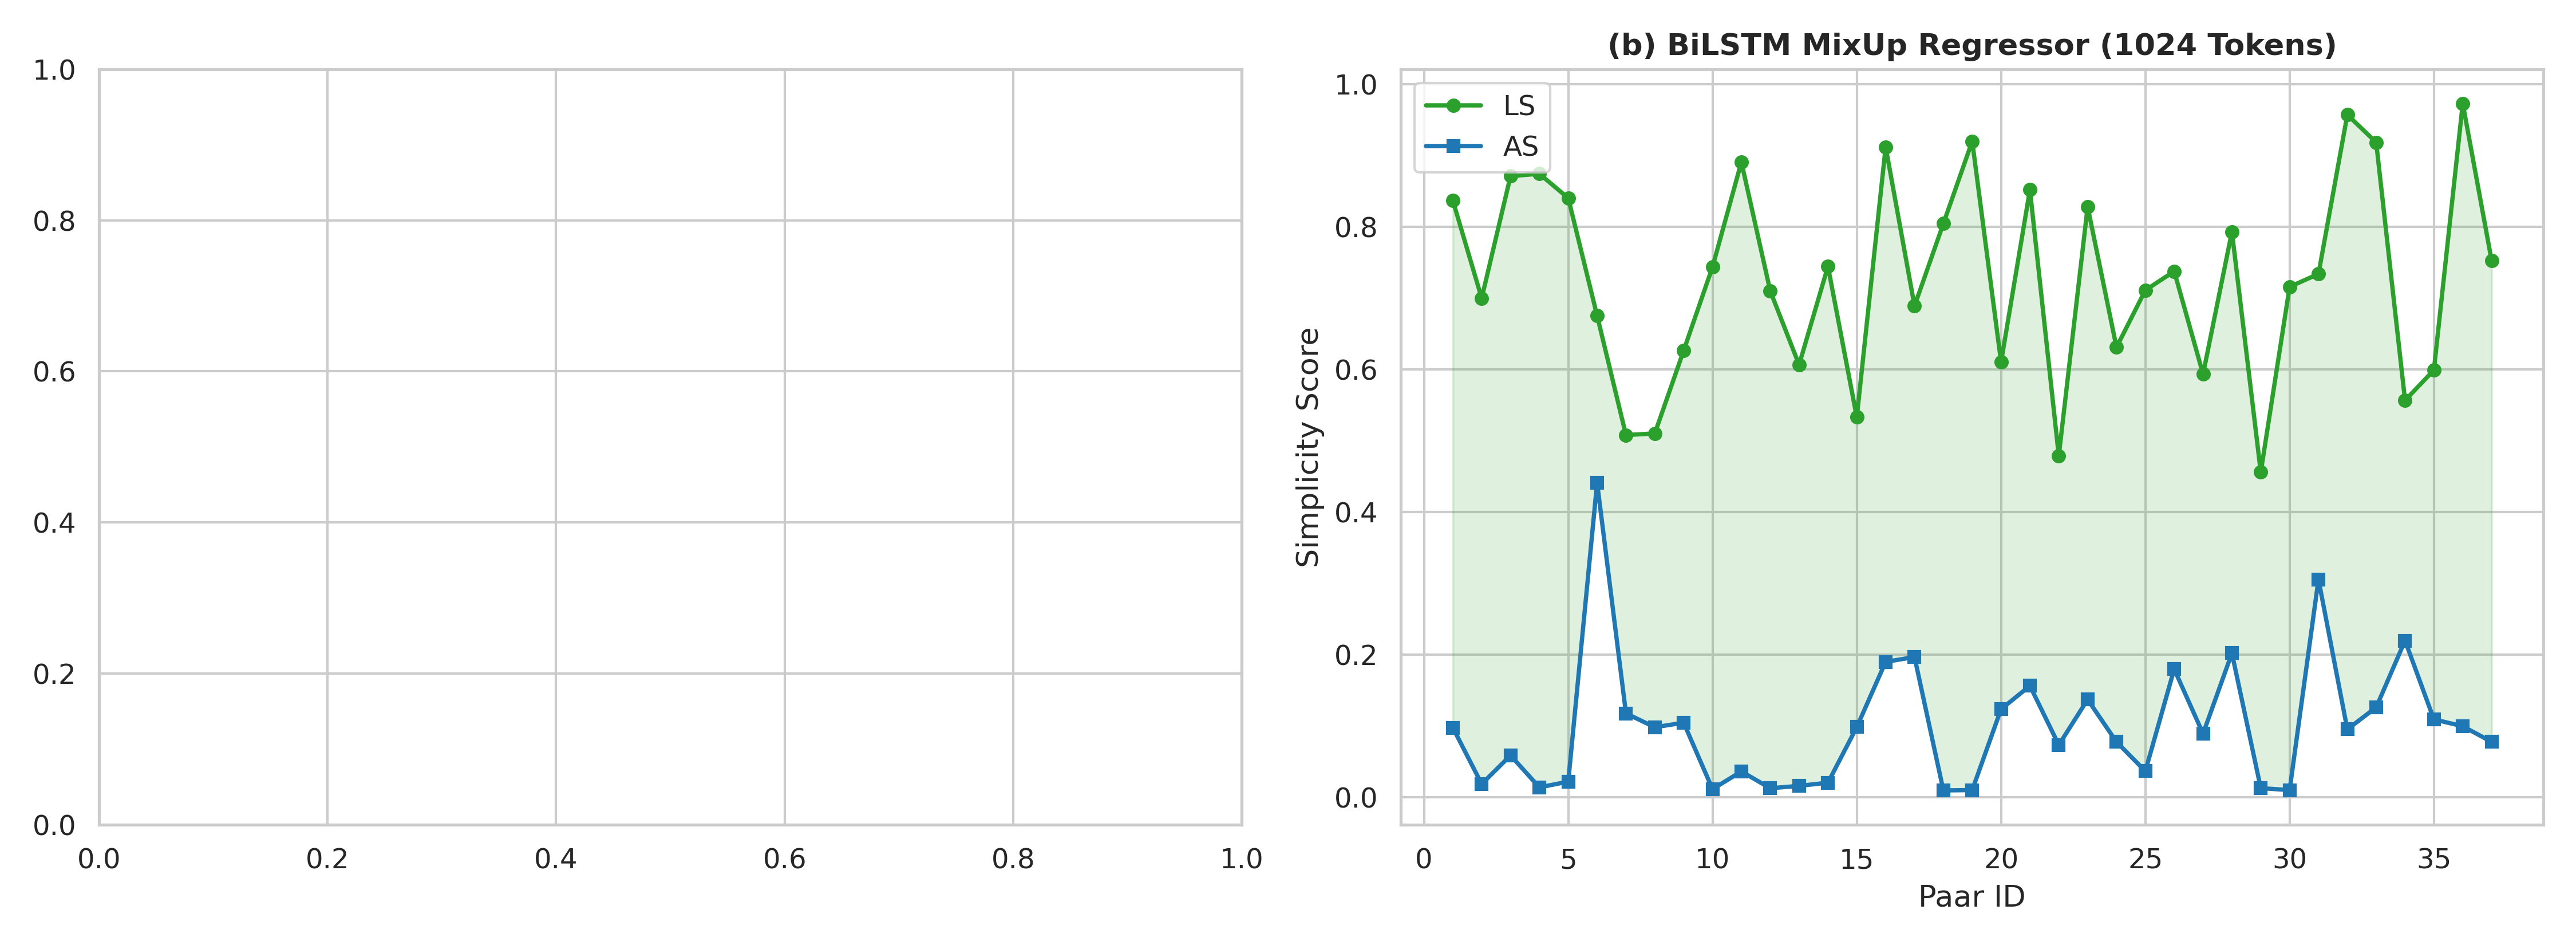
\includegraphics[width=0.95\textwidth]{images/regressor_pairwise_trajectories.png}
\caption{Paarweises Profil der Regressions-Scores und Textlängen-Einfluss: (a) Direkte Gegenüberstellung der vorhergesagten Scores für alle $37$ parallelen Lebenshilfe-Artikelpaare ($\text{LS} > \text{AS}$ bei allen Paaren, $100\,\%$ Perfect Pair Match beim $1.024$-Modell) sowie (b) Korrelation zwischen Dokumentenlänge (Satzanzahl) und resultierendem Einfachheits-Score.}
\label{fig:anhang_regressor_trajectories}
\end{figure}

\newpage
\subsection{Ergänzende Evaluation des Synthetischen Regressors \& Prompt-Design}
\label{sec:anhang_synthetic_regressor_prompt}

In diesem Abschnitt sind die ergänzenden empirischen Auswertungen zum BiLSTM Synthetischen Regressor sowie das vollständige Prompt-Design zur Erzeugung der Zwischenstufen dokumentiert.

\subsubsection{Master-Benchmark auf dem Lebenshilfe-Goldstandard}

Tabelle~\ref{tab:anhang_synthetic_vs_mixup_benchmark} stellt die Evaluierung des Synthetischen Regressors auf dem unabhängigen \textit{Lebenshilfe}-Goldstandard ($N = 37$ Artikelpaare / $74$ Dokumente, $185$ Multi-Stufen-Samples) den MixUp-Regressoren und linguistischen Formeln gegenüber.

\begin{table}[htbp]
\centering
\small
\caption{Gesamtevaluation aller Regressoren und linguistischen Baselines auf dem Lebenshilfe-Goldstandard ($N = 37$ Artikelpaare / $74$ Dokumente).}
\label{tab:anhang_synthetic_vs_mixup_benchmark}
\adjustbox{max width=\textwidth}{%
\begin{tabular}{@{}llcccccc@{}}
\toprule
\textbf{Modell} & \textbf{Ebene / Input} & \textbf{\O{} Score (LS)} & \textbf{\O{} Score (AS)} & \textbf{Separation ($\Delta$)} & \textbf{Balanced Acc} & \textbf{ROC-AUC} & \textbf{Pair Match} \\
\midrule
BiLSTM MixUp Regressor ($1.024$) & Dokument ($1.024$ Tok.) & $\mathbf{0{,}792 \pm 0{,}10}$ & $\mathbf{0{,}067 \pm 0{,}10}$ & $\mathbf{0{,}726}$ & $\mathbf{98{,}65\,\%}$ & $\mathbf{0{,}9993}$ & $\mathbf{100{,}0\,\%}\; (37/37)$ \\
BiLSTM MixUp Regressor ($512$)  & Dokument ($512$ Tok.)   & $0{,}777 \pm 0{,}12$ & $0{,}062 \pm 0{,}11$ & $0{,}715$ & $98{,}65\,\%$ & $0{,}9985$ & $97{,}3\,\%\; (36/37)$ \\
BiLSTM MixUp Regressor ($256$)  & Dokument ($256$ Tok.)   & $0{,}724 \pm 0{,}13$ & $0{,}092 \pm 0{,}09$ & $0{,}632$ & $95{,}95\,\%$ & $0{,}9982$ & $97{,}3\,\%\; (36/37)$ \\
\midrule
BiLSTM Synthetischer Regressor  & Dokument (LLM-Stufen)   & $0{,}575 \pm 0{,}35$ & $0{,}145 \pm 0{,}18$ & $0{,}429$ & $78{,}38\,\%$ & $0{,}8495$ & $89{,}2\,\%\; (33/37)$ \\
Vanilla RNN Baseline (Ablation) & Dokument ($256$ Tok.)   & $0{,}527 \pm 0{,}20$ & $0{,}287 \pm 0{,}17$ & $0{,}240$ & $81{,}08\,\%$ & $0{,}8733$ & $81{,}1\,\%\; (30/37)$ \\
\midrule
Flesch Reading Ease (Baseline)  & Dokument (Silben/Satz)  & $0{,}973 \pm 0{,}16$ & $0{,}189 \pm 0{,}39$ & $0{,}784$ & $89{,}19\,\%$ & $0{,}8919$ & $100{,}0\,\%\; (37/37)$ \\
Wiener Sachtextformel (Baseline)& Dokument (Wortlänge)    & $0{,}919 \pm 0{,}27$ & $0{,}108 \pm 0{,}31$ & $0{,}811$ & $90{,}54\,\%$ & $0{,}9054$ & $100{,}0\,\%\; (37/37)$ \\
\bottomrule
\end{tabular}}
\end{table}

\begin{figure}[htbp]
\centering
\begin{subfigure}[b]{0.48\textwidth}
    \centering
    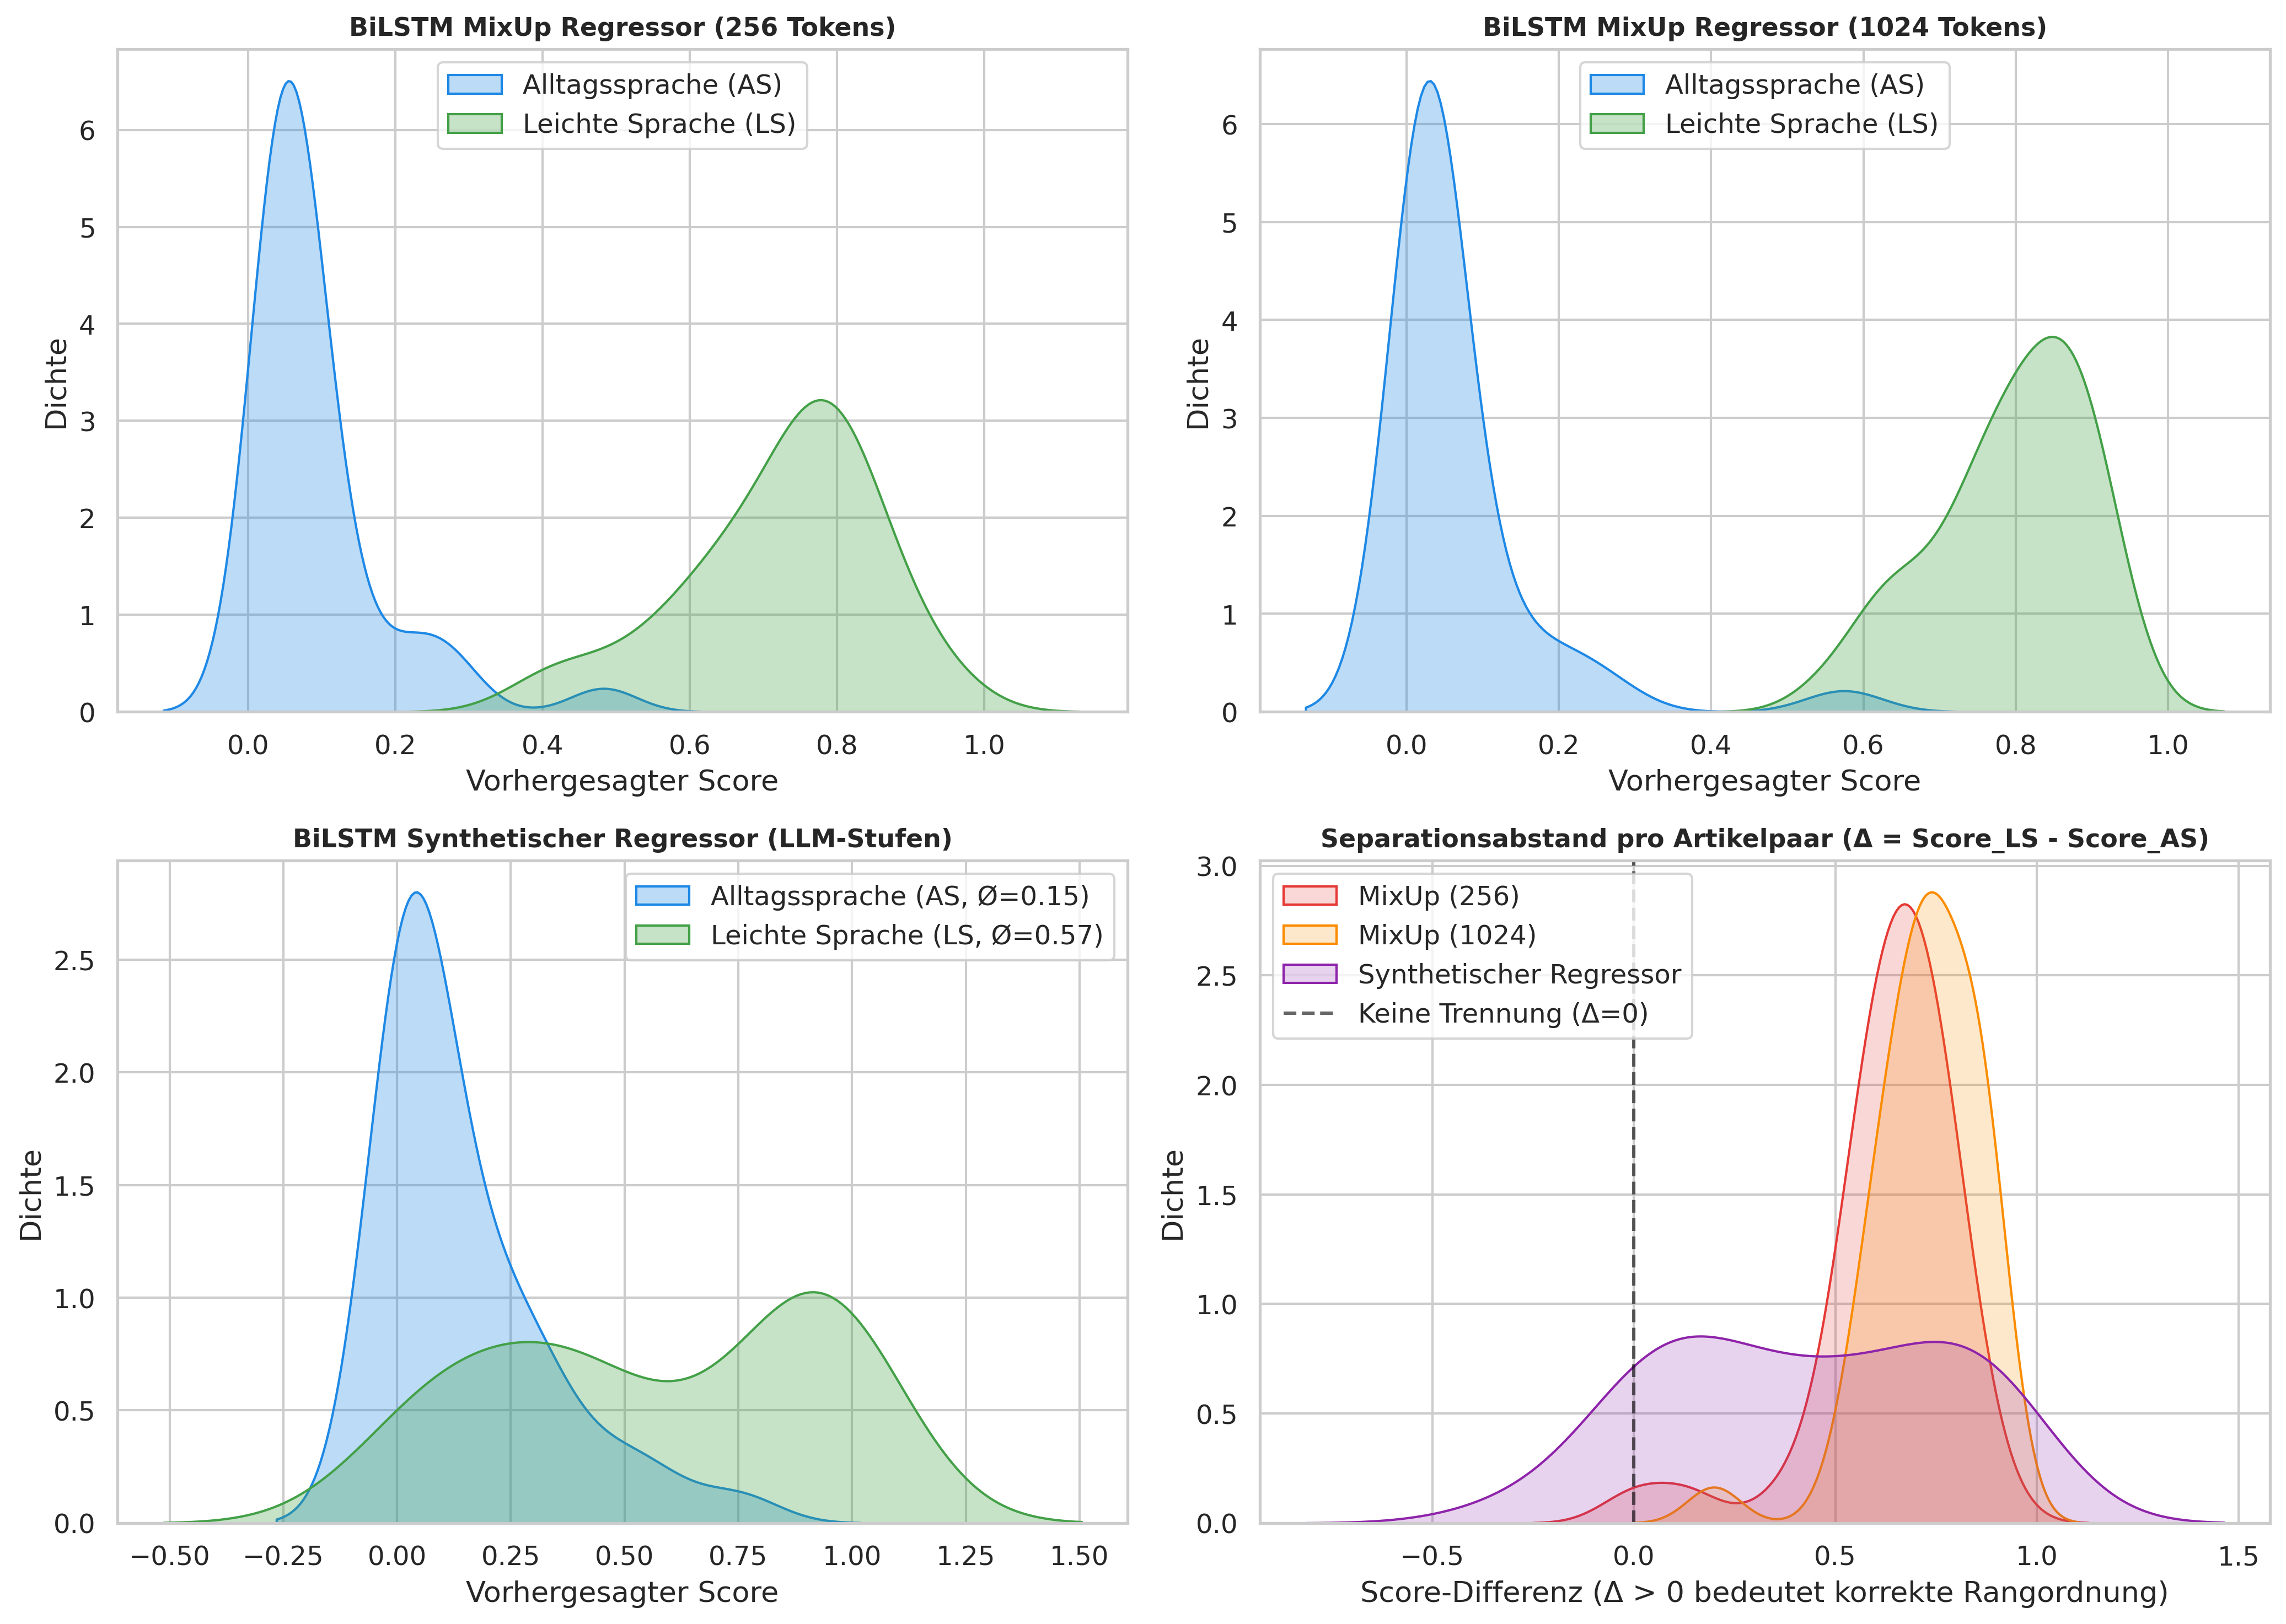
\includegraphics[width=\textwidth]{images/synthetic_regressor_kde_overview.png}
    \caption{Dichteverteilungen \& Paarseparation}
    \label{fig:anhang_synthetic_kde}
\end{subfigure}
\hfill
\begin{subfigure}[b]{0.48\textwidth}
    \centering
    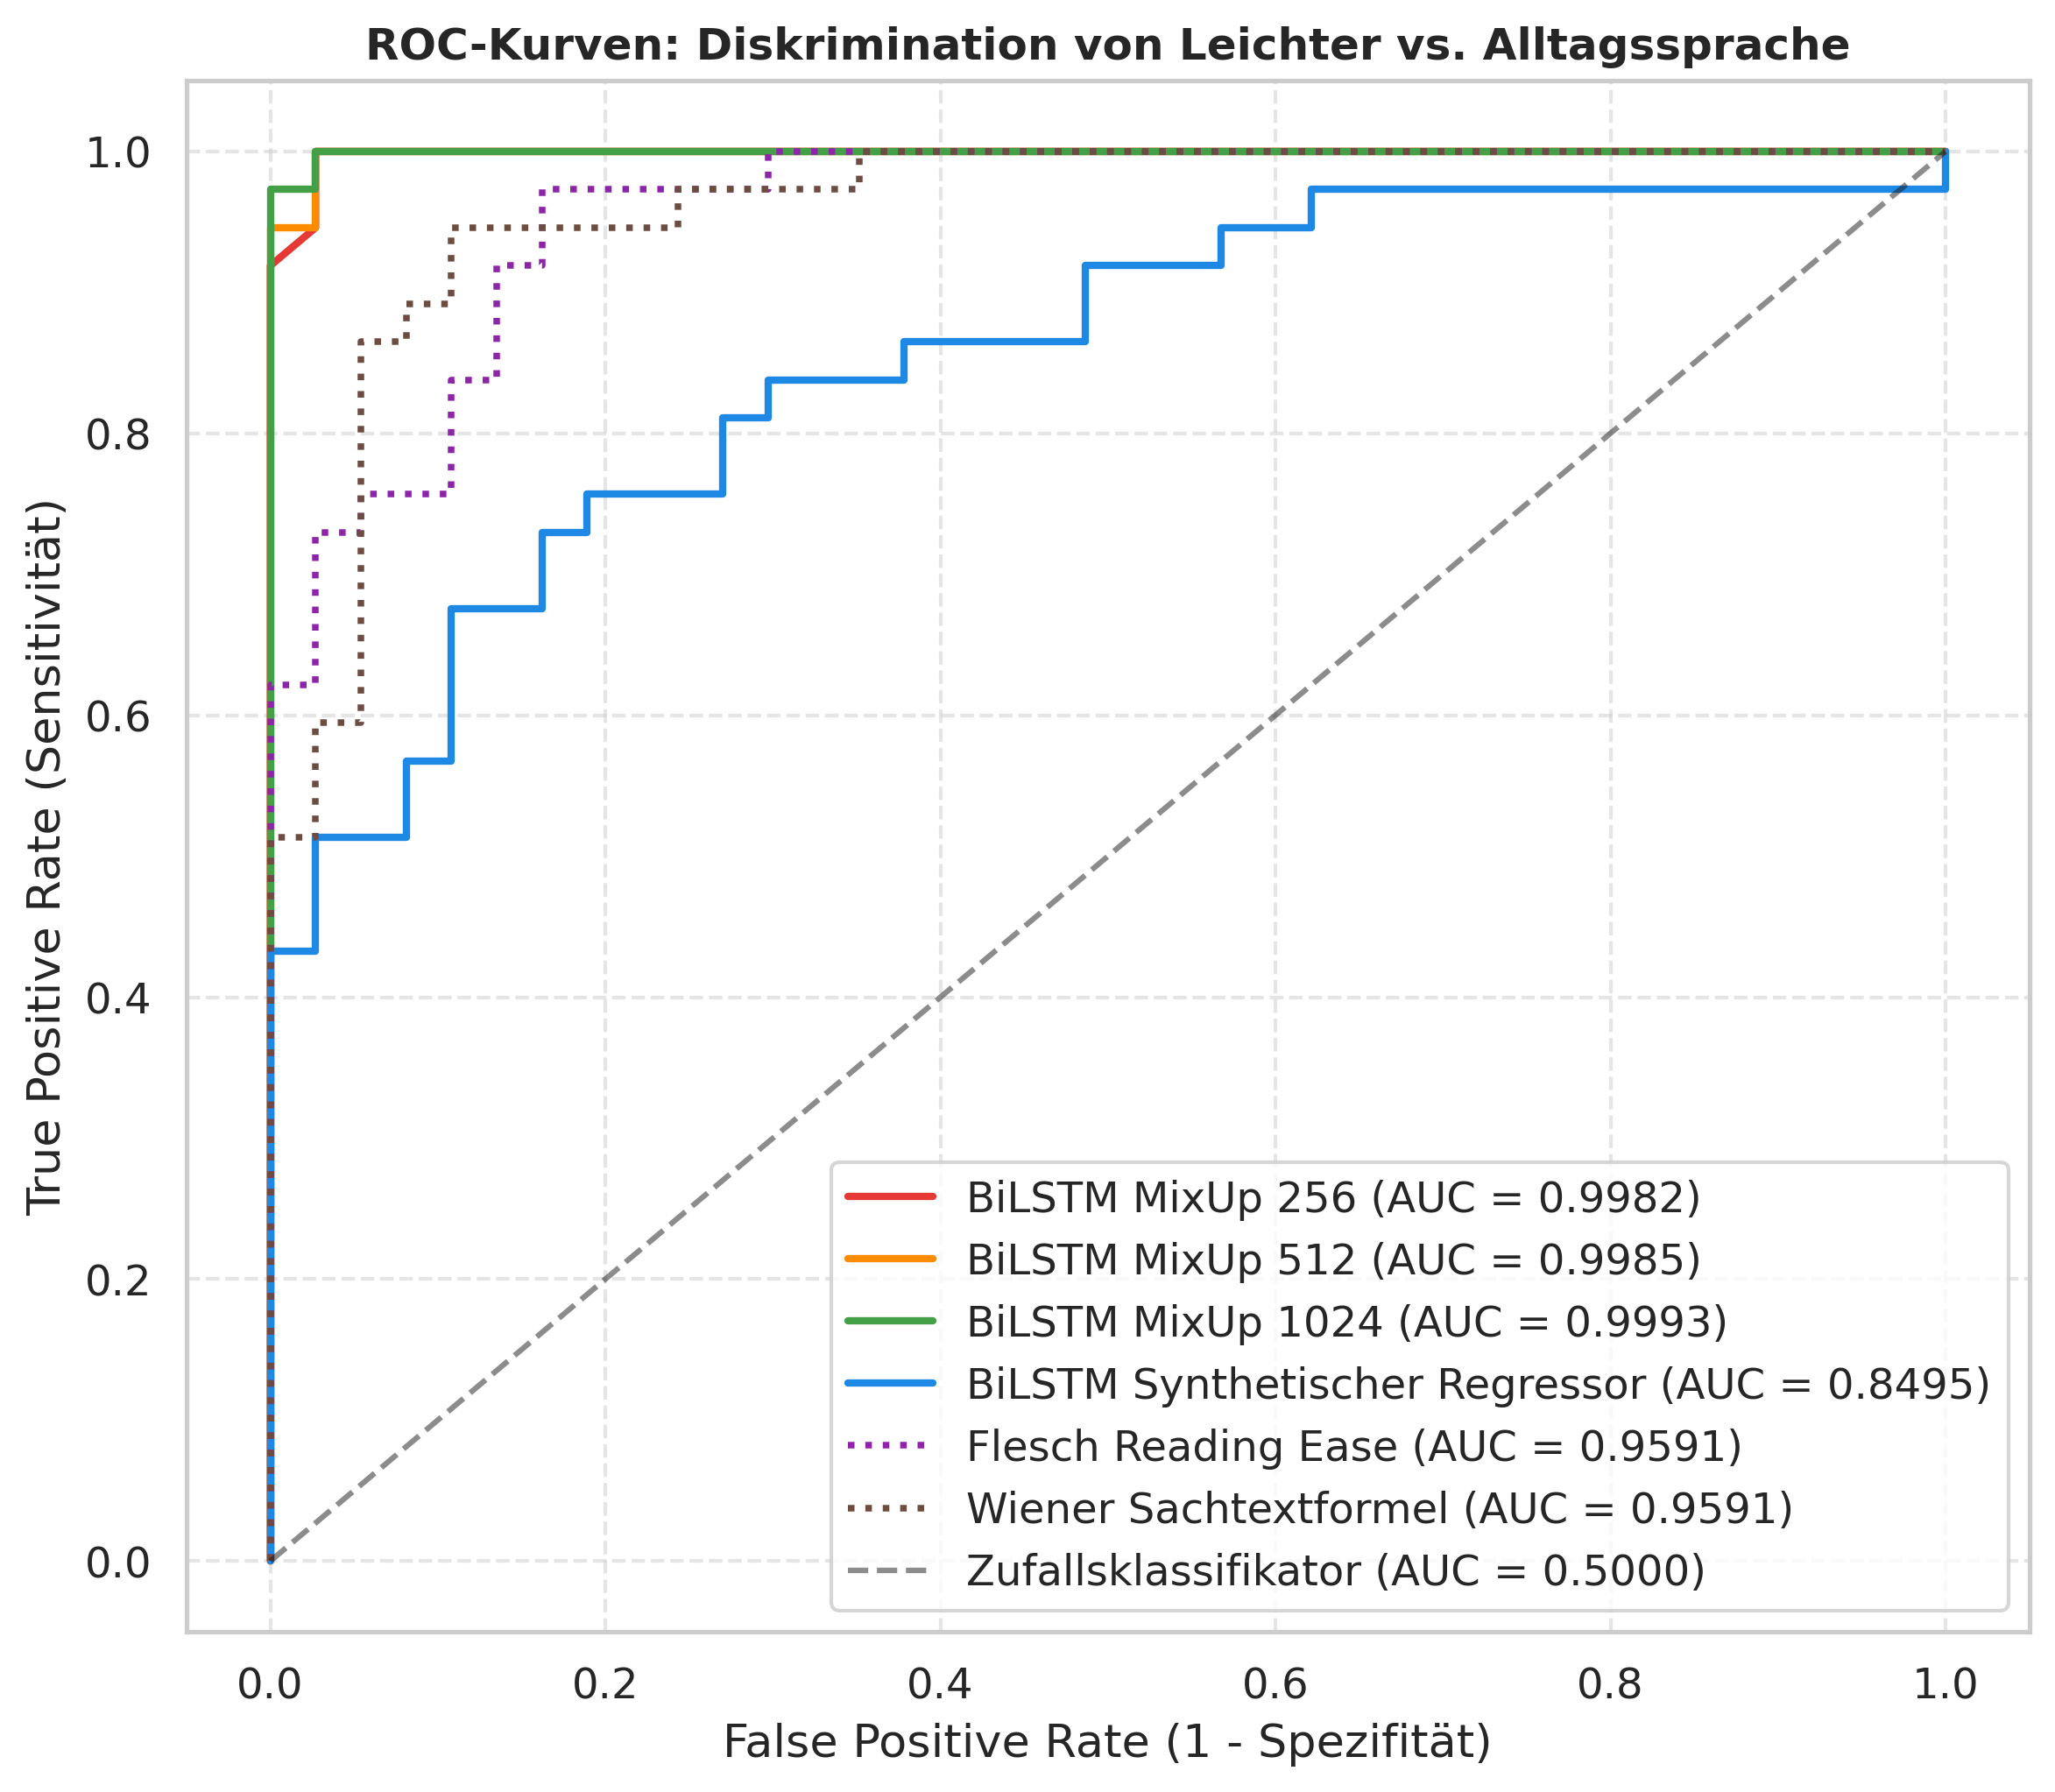
\includegraphics[width=\textwidth]{images/synthetic_regressor_roc_comparison.png}
    \caption{ROC-Kurven aller Regressoren}
    \label{fig:anhang_synthetic_roc}
\end{subfigure}
\caption{Dichteverteilungen (KDE) und Diskriminationsleistung (ROC) des Synthetischen Regressors im Vergleich zu den MixUp-Modellen und Baselines auf dem Lebenshilfe-Goldstandard.}
\label{fig:anhang_synthetic_kde_roc}
\end{figure}

\begin{figure}[htbp]
\centering
\begin{subfigure}[b]{0.48\textwidth}
    \centering
    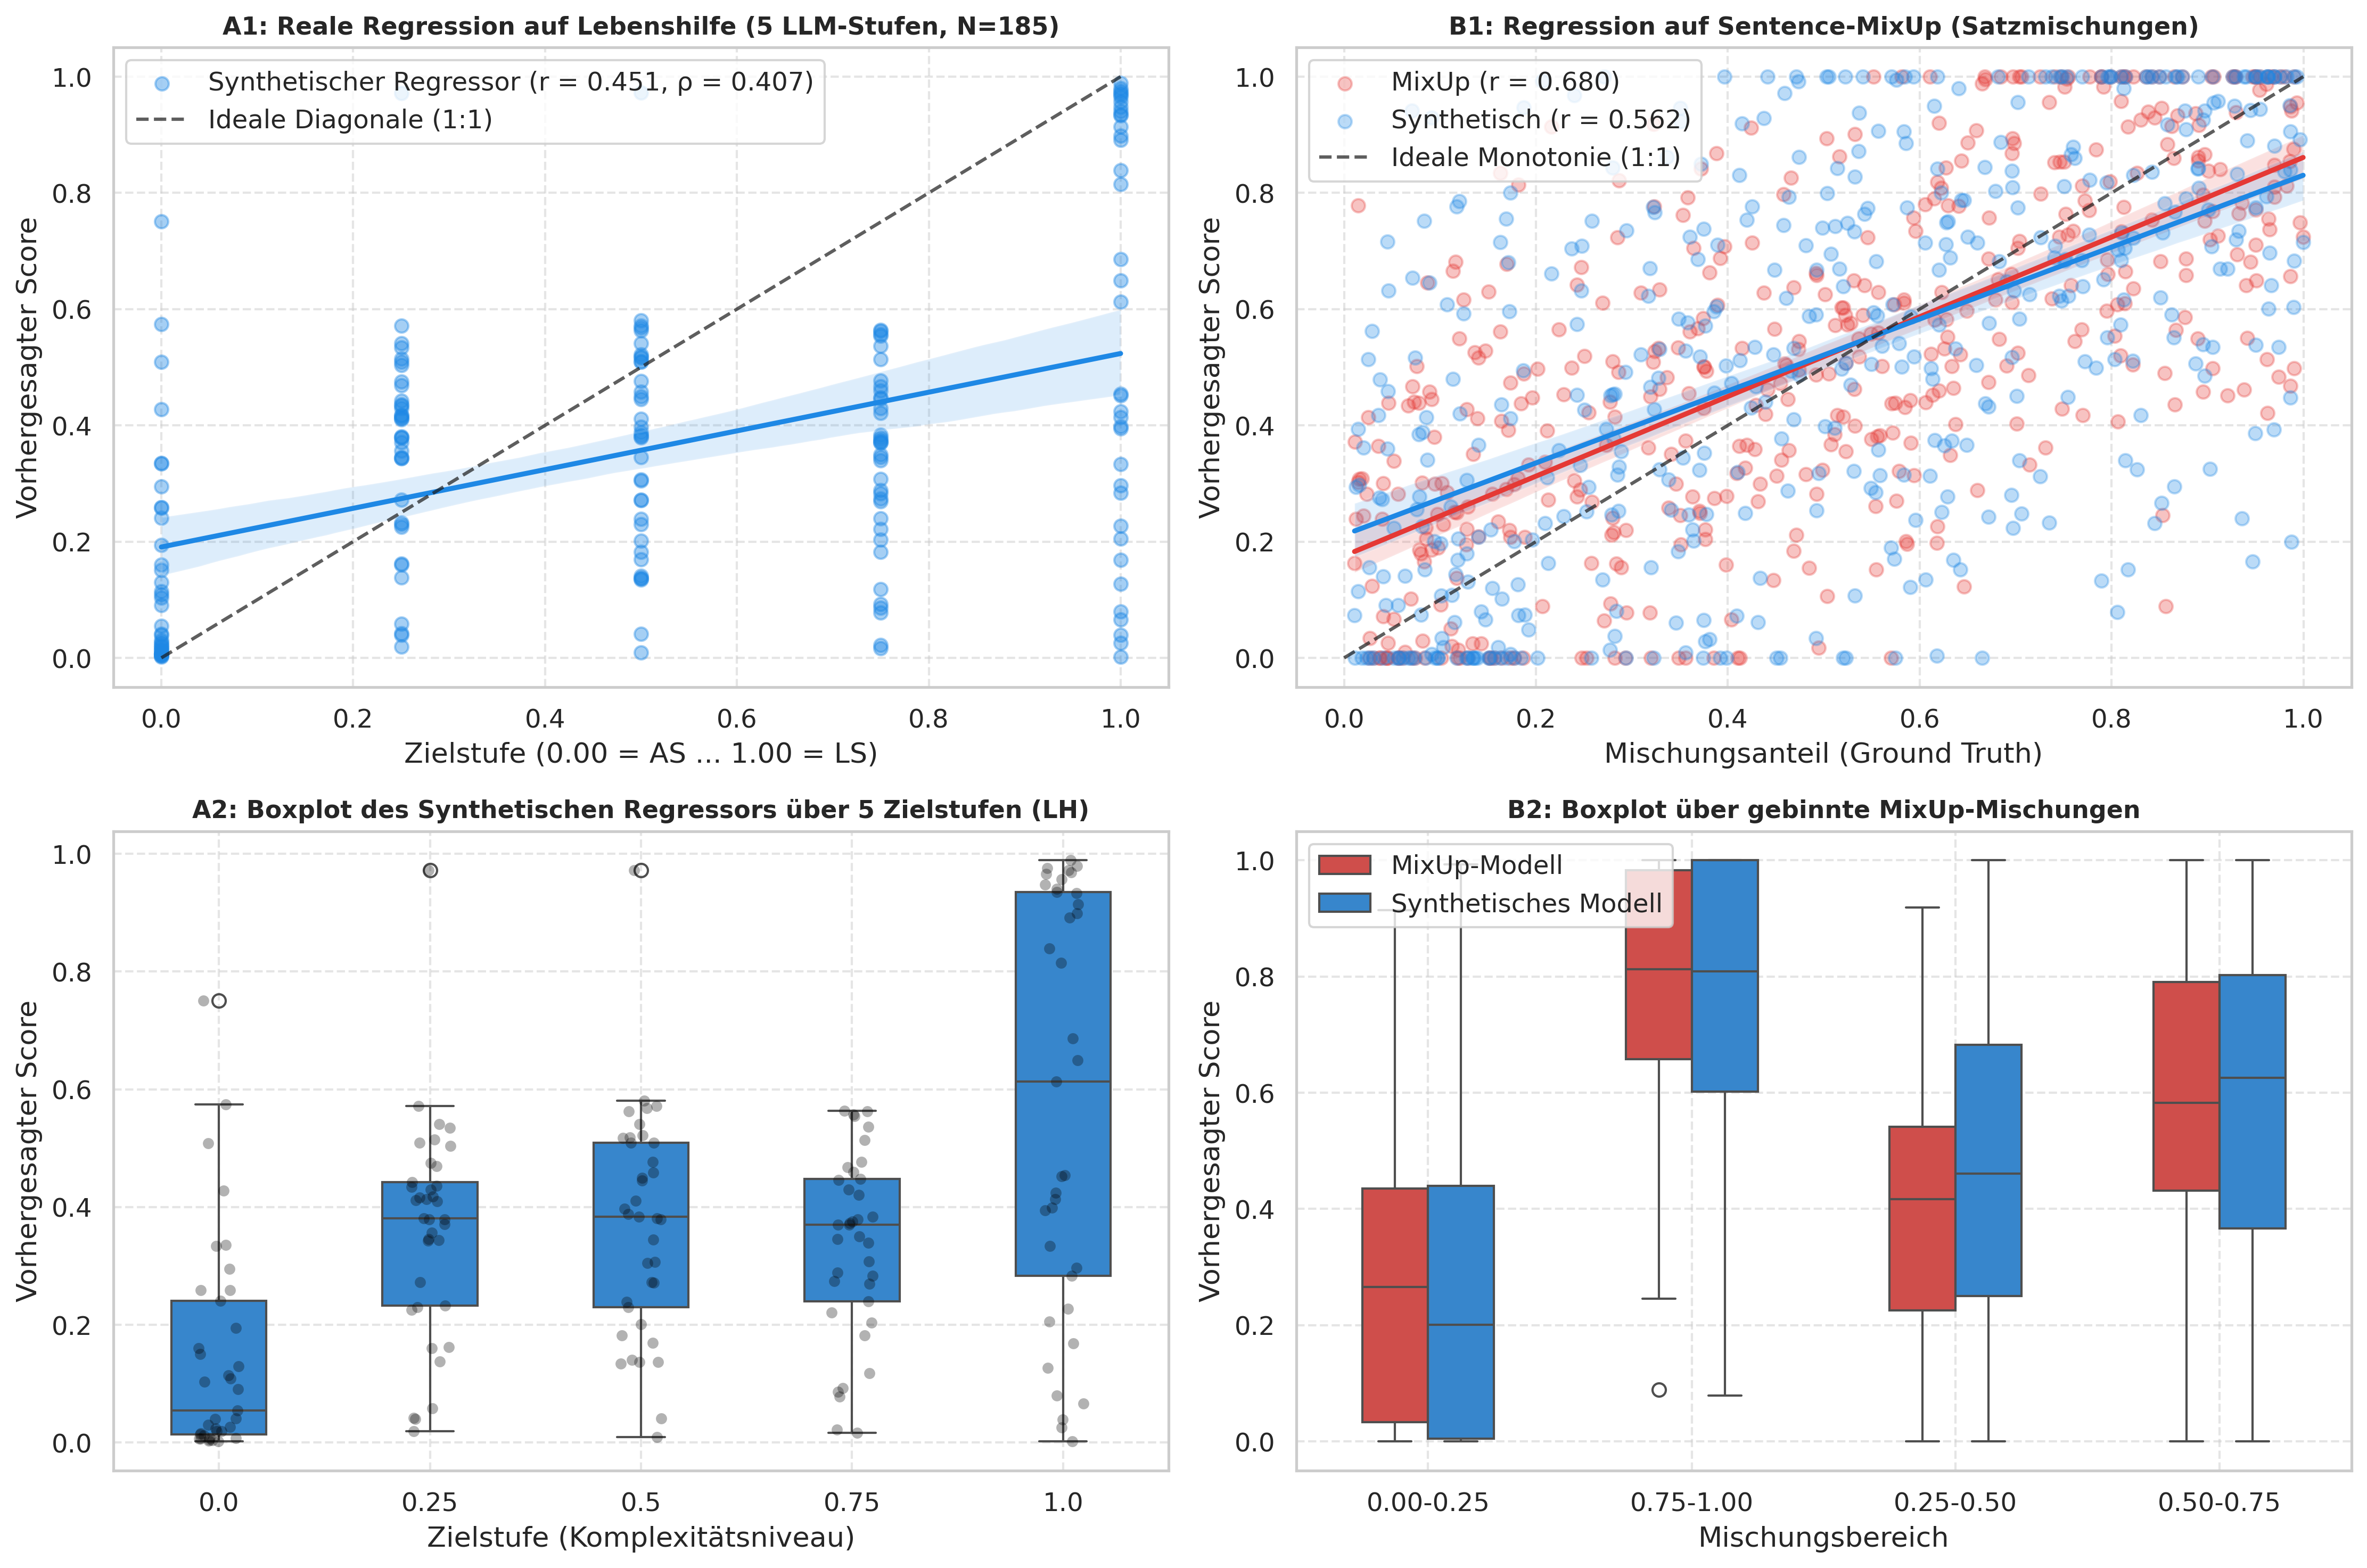
\includegraphics[width=\textwidth]{images/synthetic_regressor_regression_boxplots.png}
    \caption{Stufenmonotonie \& Boxplots}
    \label{fig:anhang_synthetic_box}
\end{subfigure}
\hfill
\begin{subfigure}[b]{0.48\textwidth}
    \centering
    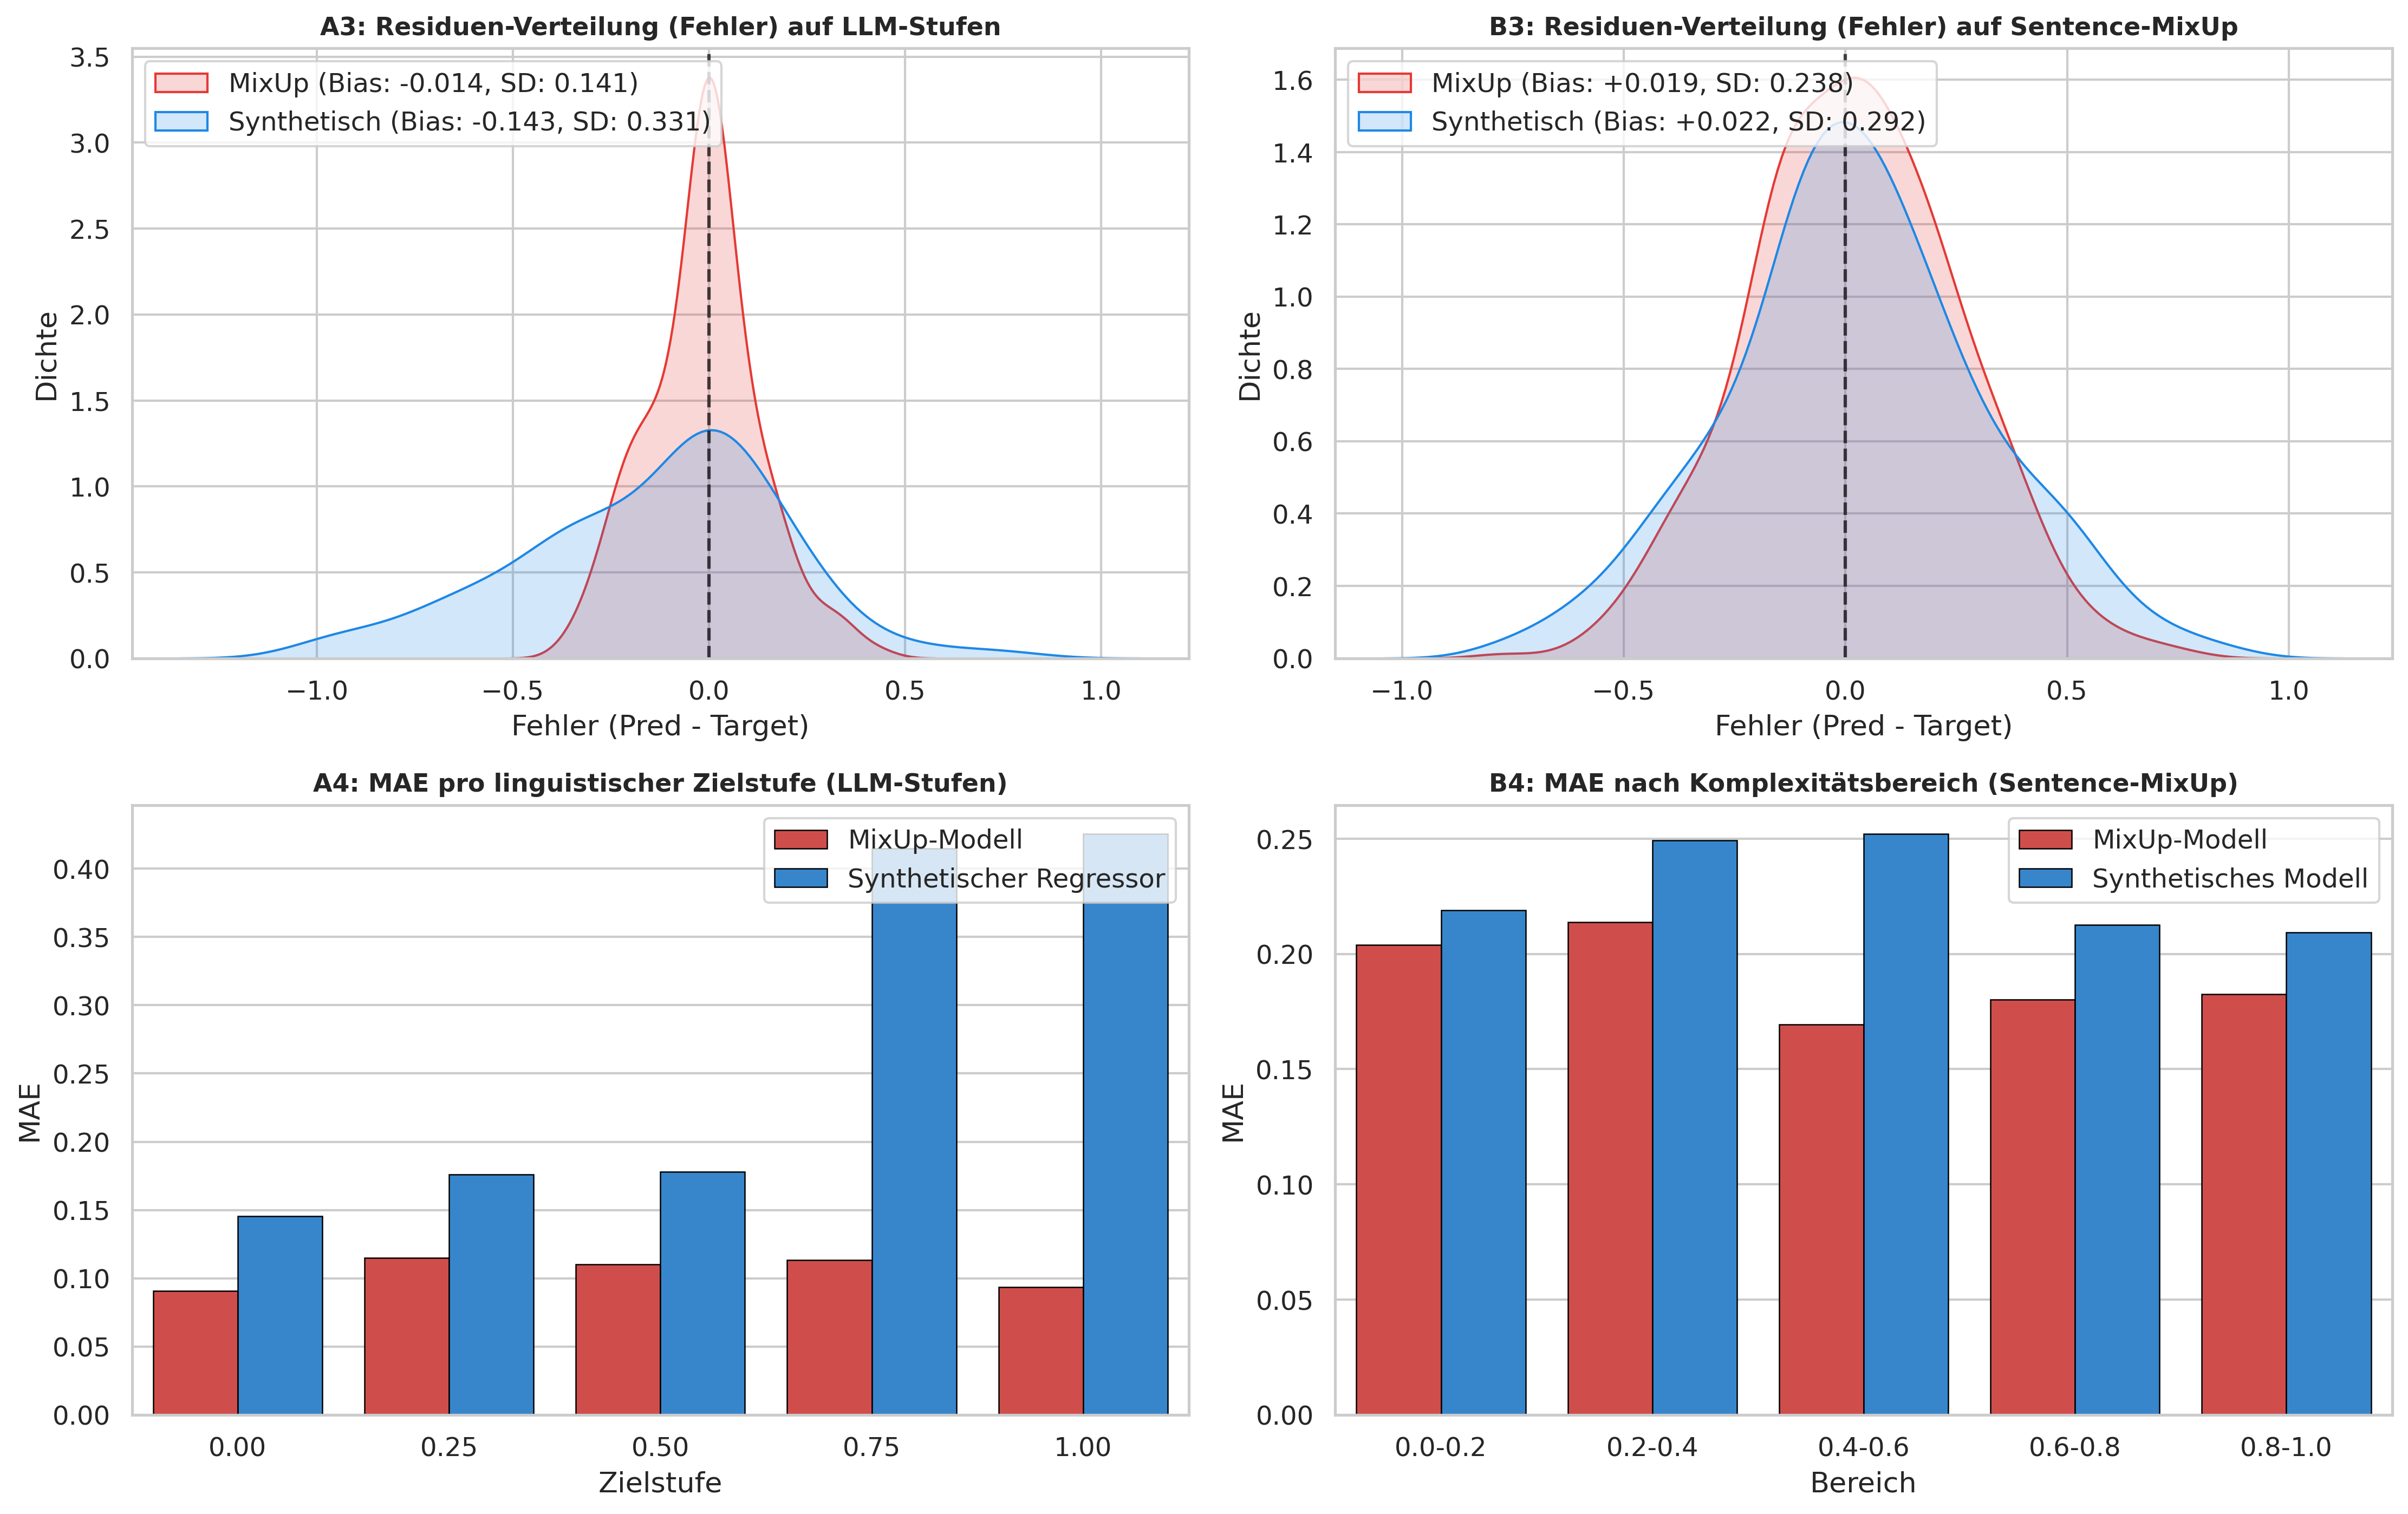
\includegraphics[width=\textwidth]{images/synthetic_regressor_residuals_mae.png}
    \caption{Residuen-Verteilung \& MAE}
    \label{fig:anhang_synthetic_mae}
\end{subfigure}
\caption{Empirische Monotonie- und Fehleranalyse des Synthetischen Regressors über die 5 diskreten LLM-Stufen auf dem Lebenshilfe-Goldstandard ($N=185$ Vorhersagen) im Vergleich zu Sentence-MixUp.}
\label{fig:anhang_synthetic_monotonie}
\end{figure}

\subsubsection{Prompt-Design zur Generierung synthetischer Zwischenstufen}

Zur Erzeugung der synthetischen Zwischenstufen ($0{,}25$, $0{,}50$, $0{,}75$) wurde das Open-Source-Modell \texttt{FlensGen-GPT-OSS-120B} (gehostet an der Hochschule Flensburg) per API mit folgender System- und User-Prompt-Struktur parametrisiert (Sampling-Temperatur $T = 0{,}2$, Top-p $0{,}95$):

\begin{tcolorbox}[colback=gray!5!white,colframe=gray!60!black,title=\textbf{System-Prompt: Synthetische Komplexitätsabstufung},sharp corners,boxrule=0.8pt]
\small\ttfamily
Du bist ein Experte für die deutsche Sprache und Textvereinfachung.\\
Dir wird ein Artikel in zwei verschiedenen Schwierigkeitsgraden vorgelegt:\\
1. Leichte Sprache (LS / Stufe 1.0): Extrem vereinfacht, kurze Sätze, sehr einfache Satzstruktur, oft mit Zeilenumbrüchen nach jedem Satzteil, geringe Wortkomplexität, keine Fremdwörter, Fachbegriffe werden direkt erklärt.\\
2. Alltagssprache (AS / Stufe 0.0): Der normale Originaltext, komplexer Satzbau, reichhaltiger Wortschatz, Nebensätze, Passiv- und Genitivkonstruktionen, Fachbegriffe.\\
\\
Deine Aufgabe ist es, eine neue Version dieses Artikels zu schreiben, die sprachlich präzise auf einer bestimmten Stufe zwischen diesen beiden Versionen liegt.\\
Die Skala reicht von 0.0 (Alltagssprache) bis 1.0 (Leichte Sprache).\\
Dir wird ein bestimmter Zielwert (z.B. 0.25, 0.50, 0.75) vorgegeben.\\
\\
Richtlinien für die Stufen:\\
- Stufe 0.75 (Nahe an Leichter Sprache):\\
\hspace*{1em}* Der Text soll sehr leicht verständlich sein.\\
\hspace*{1em}* Verwende überwiegend einfache Sätze, aber du darfst einzelne einfache Nebensätze (z.\,B. mit "weil", "wenn", "dass") einbauen.\\
\hspace*{1em}* Der Wortschatz darf minimal anspruchsvoller sein als in der LS-Version (z.\,B. geläufige Wörter anstelle von extremen Umschreibungen), aber vermeide Fremdwörter.\\
\hspace*{1em}* Informationen sollten sehr klar gegliedert sein, aber es muss nicht jeder Satzteil in einer neuen Zeile stehen.\\
\\
- Stufe 0.50 (Die goldene Mitte / Einfache Sprache):\\
\hspace*{1em}* Dies entspricht der typischen "Einfachen Sprache" (Simple Language).\\
\hspace*{1em}* Verwende eine Mischung aus kurzen und mittelschweren Sätzen.\\
\hspace*{1em}* Vermeide Schachtelsätze (mehrere Nebensätze ineinander), aber ein Hauptsatz mit einem Nebensatz ist der Standard.\\
\hspace*{1em}* Der Wortschatz ist alltäglich, ohne extreme Fach- oder Fremdwörter.\\
\hspace*{1em}* Der Text fließt natürlicher als Leichte Sprache, behält aber die gute Verständlichkeit bei.\\
\\
- Stufe 0.25 (Nahe an Alltagssprache):\\
\hspace*{1em}* Der Text ist nur leicht vereinfacht im Vergleich zur AS-Version.\\
\hspace*{1em}* Schachtelsätze werden weitgehend in zwei separate Sätze aufgeteilt.\\
\hspace*{1em}* Schwierige Fachbegriffe oder Fremdwörter werden entweder vermieden, durch geläufigere Wörter ersetzt oder im Satz kurz erklärt.\\
\hspace*{1em}* Der Satzbau ist flüssig und entspricht einem gut lesbaren Zeitungsartikel.\\
\\
Wichtige Regeln:\\
1. Verändere den Inhalt nicht: Es dürfen keine Fakten oder Informationen hinzuerfunden oder weggelassen werden, die nicht in den beiden Quelltexten vorhanden sind.\\
2. Orientiere dich stilistisch und inhaltlich an den vorgegebenen Versionen.\\
3. Gib ausschließlich den neu generierten Text zurück. Keine Metakommentare, keine Erklärungen, keine Anmerkungen, keine Markdown-Codeblöcke. Beginne direkt mit dem Text des Artikels.
\end{tcolorbox}

\begin{tcolorbox}[colback=gray!5!white,colframe=gray!60!black,title=\textbf{User-Prompt-Template: Übergabe der Artikelpaare},sharp corners,boxrule=0.8pt]
\small\ttfamily
Hier sind die beiden Versionen des Artikels:\\
\\
\#\#\# Version 1: Leichte Sprache (LS / Stufe 1.0):\\
\{ls\_text\}\\
\\
\#\#\# Version 2: Alltagssprache (AS / Stufe 0.0):\\
\{as\_text\}\\
\\
\#\#\# Ziel-Stufe: \{target\_level\}\\
\\
Erstelle nun den Text, der genau auf der Ziel-Stufe \{target\_level\} liegt. Befolge alle stilistischen Richtlinien für diese Stufe. Antworte nur mit dem generierten Text.
\end{tcolorbox}